\chapter[Perturbation theory]{Many-particle perturbation theory}

%We assume that we are considering a system with a Hamiltonian $\Ha$, containing a part $\Ha_0$ that we can write the following way
\begin{align} 
\Ha_0 &= \sum_{k,\sigma}\ep_k\cd_{k\sigma}c_{k\sigma} \qquad \text{(Fermions)} \\
\Ha_0 &= \sum_{q, \lambda}\omega_{q\lambda}\ad_{q\lambda} a_{q\lambda} \qquad \text{(Bosons)}
\end{align}
Suppose $\Ha = \Ha_0 + V$, and we want to describe the quantitative changes in observables when $\Ha = \Ha_0 \rightarrow \Ha_0 + V$, when we cannot solve the problem with $V\ne 0$ exactly. One then has to resort to more or less systematic approaches.

\underline{Examples of V:}
\begin{enumerate}[i)]
	\item \[V = \sum_{k,q,\sigma}g_{q\lambda}\left( a_{-q,\lambda}^\dagger + a_{q,\lambda} \right)\cd_{k+q,\sigma}c_{k,\sigma}\]
	\item \[V=\sum_{\substack{k,k',q \\ \sigma,\sigma'}}\tilde{V}(q)\cd_{k+q,\sigma}\cd_{k'-q, \sigma'}c_{k'\sigma'}c_{k\sigma}\]
	\item Hubbard-interaction
	\item etc
\end{enumerate}

\section{Time-evolution of states}

\begin{enumerate}[i)]
	\item \underline{Schrödinger-picture:} 
	
	Operators are time-independent. States are time-dependent.
	\begin{align*} 
	\hat{O}(t) &= \hat{O}(0) \\
	i\dv{\ket{\psi}}{t} &= \Ha\ket{\psi} \\
	\ket{\psi(t)} &= \e^{-\Ha t}\ket{\psi(0)}
	\end{align*}
	
	\item \underline{Heisenberg-picture}:
	
	Operators are time-dependent. States are time-independent
	\begin{align} 
	\hat{O}(t) &= \e^{i\Ha t}\hat{O}(0)\e^{-i\Ha t} \\
	\ket{\psi(t)} &= \ket{\psi(0)}
	\end{align}		
\end{enumerate}
Notice that $\mel{\psi(0)}{\hat{O}(t)}{\psi(0)} = \mel{\psi(t)}{\hat{O}(0)}{\psi(t)}$, i.e Matrix-elements are the same in both the Heisenberg- and Schrödinger-picture.
This suggests a considerable degree of freedom in choosing how to time-evolve operators and states, and the choice is to some extent dictated by convenience. 
For developing a (in principle!) systematic perturbation theory for observables in many-body systems, it turns out that a picture which is a hybrid of the Schrödinger- and Heisenberg picture, is convenient. In this picture ``most of'' the time-evolution the time-evolution is put in the operators, and  ``a little bit'' of the time-evolution is put in the states; 
\begin{align}
\label{eq:interaction_picture}
\begin{split} 
O(t) &= \e^{i\Ha_0 t}\hat{O}(0)\e^{-i\Ha_0 t} \\[2ex]
\ket{\psi(t)} &= \e^{i\Ha_0 t}\e^{-i\Ha t}\ket{\psi(0)}.
\end{split}
\end{align}

The relations in \cref{eq:interaction_picture} give the same matrix-elements as in the Schrödinger and Heisenberg pictures. 
The non-trivial operator evolving $\ket{\psi(t)}$ is
\begin{align} 
U(t) &= \e^{i\Ha_0 t}\e^{-i\Ha t} \\[2ex]
\ket{\psi(t)} &= U(t)\ket{\psi(0)}.
\end{align}
 We would, ideally, like to establish a perturbation series in $V$ in $U$. 
 Note that in general, $\comm{\Ha_0}{V}\ne 0$ such that \[\e^{-\Ha_0 t}\e^{i\Ha t}\ne \e^{-iV t}!\]
 
 Proceed as follows: 
 
 \begin{align*} 
 \dv{U(t)}{t} &=  i\Ha_0\e^{i\Ha_0 t}\e^{-i\Ha t}- i\e^{i\Ha_0 t}\e^{-i\Ha t}\Ha \\
 &= i \e^{i\Ha_0 t}\underbrace{\left( \Ha_0 - \Ha \right)}_{-V}e^{-i\Ha t} \\
 &= -i \underbrace{\e^{i\Ha_0 t}V\e^{-i\Ha_0 t}}_{V(t)}\underbrace{\e^{i\Ha_0 t}\e^{-i\Ha t}}_{=U(t)} \\
 &= -iV(t)U(t) \\
 \int_{\tilde{t}}^{t}\dd{t'} \dv{U(t')}{t'} &= -i\int_{\tilde{t}}^{t}\dd{t'}V(t')U(t') \\
 U(t) &= U(\tilde{t}) -i \int_{\tilde{t}}^{t}\dd{t'}V(t')U(t') \\
 U(0) &= 1, \quad \text{Choose } \tilde{t} =0 \\
 U(t) &= 1 -i\int_0^t\dd{t}V(t')U(t')
 \end{align*}
 This equation can be solved by iteration to generate a power seris in V. This is essentially what we will do, but before doing so, it will be convenient to introduce a slightly more general evolution-operator.
 
\section{The S-matrix}

The S-matrix is defined as follows:
\begingroup
\addtolength{\jot}{1em}
\begin{align*}
\ket{\psi(t)} &= S(t, t')\ket{\psi(t')} \\
S(t,0) &= U(t)\\
\ket{\psi(t)} &= S(t, t')U(t')\ket{\psi(0)} \\
U(t) &= S(t, t')U(t') \\
S(t, t') &= U(T)U^{-1}(t')
\end{align*}
\endgroup
Using that $U^\dagger = U^{-1}$ (by the definition of $U$) we get
\begin{equation} 
S(t, t') = U(t)U^\dagger (t')
\end{equation}

Some properties of $S$:
\begin{enumerate}[i)]
	\item \[S(t, t') = 1\]
	\item \begin{equation}\label{eq:S_prop} 
	S^\dagger(t, t') = S(t', t)
	\end{equation}
	\item \begin{align*} 
	\ket{\psi(t)} &= S(t, t')\ket{\psi(t')} \\
	&=  S(t, t')S(t', t'')\ket{\psi(t'')} \\
	&=  S(t, t'')\ket{\psi(t'')}
	\end{align*}
	\begin{equation} 
	\label{eq:S_matrix}
	S(t, t'') = S(t, t')S(t', t'')
	\end{equation}
\end{enumerate}

The equation for $S$ is
\begin{align*} 
\pdv{S(t, t')}{t} &= \pdv{U}{t}U^\dagger(t') \\
&= -V(t)U(t)U^\dagger(t') \\
&= -iV(t)S(t, t') \\
\int_{\tilde{t}}^{t}\dd{t''}\pdv{S}{t''} &= -i\int_{\tilde{t}}^{t}\dd{t''}V(t'')S(t'', t') \\
S(t, t') &= S(\tilde{t}, t') -i \int_{\tilde{t}}^{t}V(t'')S(t'', t')
\end{align*}
Now choose $\tilde{t} = t'$ and use that $S(t',t') = 1$ to obtain
\begin{equation}
\label{eq:S_matrix_eq}
S(t, t'') = 1-i\int_{t'}^t\dd{t''}V(t'')S(t'', t')
\end{equation}
This we will solve by iteration to produce a power series in $V$ for $S$. This power-series for $S$ will then generate a power-series in $V$ for any observable.


\underline{\textbf{Iteration:}}

\begin{enumerate}
	\item[\underline{0th order:}] \[S_0('t, t') = 1\]
	\item[\underline{1st order:}] \begin{align*} 
		S_1(t, t') &= 1-i\int_{t'}^{t}\dd{t''}V(t'')S_0(t'', t') \\
		&= 1-i\int_{t'}^{t}\dd{t''}V(t'')	
	\end{align*}
	\item[\underline{2nd order:}] 
	\begin{align*} 
	S_2(t, t') &= 1-i\int_{t'}^{t}\dd{t''}V(t'')S_1(t'', t') \\
	&= 1 + (-i)\int_{t'}^{t}\dd{t''}V(t'') + (-i)^2\int_{t'}^{t}\dd{t''}V(t'')\int_{t'}^{t''}\dd{t'''}V(t''')
	\end{align*}
	
	\item[\underline{Infinite order:}]
	\begin{equation} \label{eq:S_power_series}
	S(t, t') = 1 + \sum_{n=1}^\infty(-i)^n\int_{t'}^{t}\dd{t_1}\int_{t'}^{t_1}\dd{t_2}\cdots\int_{t'}^{t_{n-1}}\dd{t_n}V(t_1)\cdots V(t_n)
	\end{equation}
\end{enumerate}
Note: Lower integration limits are all the same, but the upper ones are different. We will now transform this integral into one where also all upper limits are the same, by introducing the time-ordering operator.
$\tilde{T}: $ time-ordering operator for fermions.
\begin{equation}
\tilde{T}\left[A(t_1)B^\dagger(t_2)\right] =  
\begin{cases}
A(t_1)B^\dagger(t_2),\quad t_1>t_2 \\
-B^\dagger(t_2)A(t_1), \quad t_2>t_1
\end{cases}
\end{equation}
Consider now the second-order in $V$-term in \cref{eq:S_power_series}, and work backwards, starting with 
\[\frac{1}{2!}\int_{t'}^{t}\dd{t_1}\int_{t'}^{t}\dd{t_2}\tilde{T}[V(t_1)V(t_2)].\]
For $V(t)$, we assume that it is composed of fermion- or boson-operators in such a way that \begin{equation} 
\tilde{T}[V(t_1)V(t_2)] = \begin{cases}
V(t_1)V(t_2),\quad t_1>t_2 \\
V(t_2)V(t_1),\quad t_2>t_1
\end{cases}
\end{equation}

\begin{align*} 
\frac{1}{2!}&\int_{t'}^{t}\dd{t'}\int_{t'}^{t_1}\dd{t_2}V(t_1)V(t_2)\\
&+\frac{1}{2!}\int_{t'}^{t}\dd{t_1}\int_{t_1}^{t_2}\dd{t_2}V(t_2)V(t_1)
\end{align*}
Now let $t_1 \leftrightarrows t_2$ in the second term
\begin{equation} 
\implies  \int_{t'}^{t}\dd{t_1}\int_{t'}^{t_1}\dd{t_2}V(t_1)V(t_2) = \frac{1}{2!}\int_{t'}^{t}\dd{t_1}\int_{t'}^{t}\dd{t_2}\tilde{T}[V(t_1)V(t_2)]
\end{equation}
In the same way, 

\begin{align}
\begin{split} 
\frac{1}{n!}\int_{t'}^{t}\dd{t_1}\int_{t'}^{t}\dd{t_2}\cdots \int_{t'}^{t}\dd{t_n}\tilde{T}[V(t_1)\cdots V(t_2)] \\[2ex]
=\int_{t'}^t\dd{t_1}\cdots\int_{t'}^{t_{n-1}}\dd{t_n}V(t_1)\cdots V(t_n)
\end{split}
\end{align}
Thus, we have for $S(t,t')$
\begin{align} 
\nonumber
S(t, t') &= 1 + \sum_{n=1}^{\infty}\frac{(-i)^n}{n!}\int_{t'}^{t}\dd{t_1}\cdots\int_{t'}^{t}\dd{t_n}\tilde{T}[V(t_1)\cdots V(t_n)] \\[2ex]
&= 1 + \tilde{T}\left\{\sum_{n=1}^{\infty}\frac{(-i)^n}{n!}\left[\int_{t'}^{t}\dd{t''}V(t'')\right]^n \right\}\nonumber \\[2ex]
&\implies S(t, t') = \tilde{T}\qty[\exp{\displaystyle -i\int_{t'}^{t}\dd{t''}V(t'')}]. \label{eq:s_matrix}
\end{align}
Typically, what we want to compute is some matrix-element of the form 

\begin{align}
\nonumber
%\begin{split}[2]
&\ev{\hat{O}(t)}{\psi(0)} & \text{Heisenberg-picture} \\[2ex] \label{eq:pictures}
= &\ev{\hat{O}(0)}{\psi(t)} & \text{Schrödinger-picture} \\[2ex]
= &\ev{O(t)}{\psi(t)} & \text{Interaction-picture}
%\end{split}
\nonumber
\end{align}

where $\hat{O}$ is an operator representing som observable. The main problem is that $\ket{\psi}$ is unknown. What we know how to find, is $\Phi_0$ by
\begin{equation} 
\Ha_0\ket{\Phi_0} = E_0\ket{\Phi_0}.
\end{equation}
$\ket{\Phi_0}$: Eigenstate of the non-interacting system. The idea now is to replace $\ev{\hat{O}}{\psi}$ with $\ev{\hat A}{\Phi_0}$, where we at least can find a power series in $V$ for $\hat{A}$.  Since $\Phi_0$ is known, the necessary matrix-elements can be computed. It is the $S$-matrix that will facilitate this replacement. So we need to relate $\psi$ and $\Phi_0$. 

Imagine that at $t = -\infty$ (distant past, ``way before the dinosaurs''), $V(t) = 0$. Then $\Ha = \Ha_0$, $\Ha\ket{\psi} = \Ha_0\ket{\psi} = E_0\ket{\Phi_0}$.
\[\ket{\psi(-\infty)} =\ket{\Phi_0}.\]
Next, bring in perturbation adiabatically. \[\Ha = \Ha_0 + V\e^{-\ep|t|}\]
For $|t|<<\ep^{-1}, \Ha = \Ha_0 +V$, while for $|t|>>\ep^{-1}, \Ha = \Ha_0$.
\begin{figure}
	\centering
	\begin{tikzpicture}[scale=1]

\begin{axis}[
ticks = none,
legend style={font =\Large,at={(1,0.3)}},
%ytick = {1},
%yticklabels = {$\varepsilon_f$},
%xtick = {0},
%xticklabels ={,,},
xlabel = \Large $t$,
axis lines = center,
x label style={at={(axis description cs:1,0.1)}, anchor = west},
ymin = 0,
ymax= 2,
%xmax = 2.5,
%axis x line shift = -1.5
y label style={at={(axis description cs:0.5,1)},rotate=0,anchor=east},
%xlabel = $x$,
ylabel = \Large {$\Ha$},
]
%%Below the red parabola is defined
%\addplot [
%thick,
%domain=0:1.4, 
%samples=100, 
%color=red,
%]{1/2 * (1 + x^2 + sqrt((x^2 - 1)^2 + 0.1))};

%\coordinate (b) at (axis cs:1,0) ;
%\node[circle, fill, inner sep =1.8pt] at (b){};
%\node[anchor = north] at (axis cs:1.05,-0.1){\Large $k_F$};

\addplot [dashed,
thick,
domain=-3:3, 
samples=100, 
color=green!50!black,
]{1 + 0*x};

%Here the blue parabloa is defined
\addplot [
thick,
domain=-3:3, 
samples=100, 
color=blue,
]{1 + 0.5*exp(-0.2 * abs(x^2))};


\addplot +[name path = a,mark = none] coordinates {(-0.2,0) (-0.2,1.9)};
\addplot +[name path = b,mark = none] coordinates {(0.2,0) (0.2,1.9)};
\addplot[gray, pattern=north west lines] fill between[of=a and b];

\addlegendentry{${\Ha_0}$};
%\addlegendentry{$\Ha_0 + V\e^{-\ep |t|}$};
\end{axis}
\end{tikzpicture}
	\caption{The shaded region represents the time interval of interest.}
	\label{fig:adiabatic}
\end{figure}

\begin{equation} 
\ket{\psi(t)} = S(t, -\infty)\ket{\Phi_0}
\end{equation}
What is $\ket{\psi(+\infty)}$? In the interaction picture, we have
\begin{equation}
\label{eq:mel}
\ev{O(t)}{\psi(t)} = \ev{S(-\infty, t)O(t)S(t, -\infty)}{\Phi_0}
\end{equation}
If the leftmost factor of $S$ had been $S(+\infty, t)$, then $SO(t)S$ would have been time-ordered. Therefore, we will try to bring in $S(+\infty, t)$ on the left, instead of $S(-\infty, t)$. We do this as follows:
\begin{align*} 
\ket{\psi(\infty)} &= S(\infty, -\infty)\ket{\psi(-\infty)} \\
&=S(\infty, -\infty)\ket{\Phi_0} \\
&= \e^{iL}\ket{\Phi_0} \\
\braket{\Phi_0}{\Phi_0} &= 1 \\
 \implies \e^{iL} &= \braket{\Phi_0}{\psi(+\infty)}\\
&=\ev{S(\infty, -\infty)}{\Phi_0}\\
\ket{\psi(-\infty)} &= S(-\infty, \infty)\ket{\psi(+\infty)},
\end{align*}
where \cref{eq:S_prop} was used in the last step. 

\textbf{NB:} \[\ket{\Phi_0}= \e^{iL}S(-\infty, \infty)\ket{\Phi_0}.\]
Now, we have what we need! By inserting $\bra{\Phi_0}= \e^{-iL}\bra{\Phi_0}S(\infty, -\infty)$ in \cref{eq:mel}, we get
\begin{equation*} 
\ev{S(-\infty, t)O(t)S(t, -\infty)}{\Phi_0} = \e^{-iL}\ev{S(+\infty, t)O(t)S(t, -\infty)}{\Phi_0}
\end{equation*}
and finally 
\begin{equation}
	\ev{O(t)}{\psi(t)} = \frac{\ev{S(+\infty, t)O(t)S(t, -\infty)}{\Phi_0}}{\ev{S(\infty, -\infty)}{\Phi_0}}
\end{equation}
with \[O(t) = \e^{i\Ha_0 t}\hat{O}(0)\e^{-i\Ha_0 t}\] (as in \cref{eq:interaction_picture}).
Perturbation-expansion for $S \implies$ perturbation-expansion for matrix-element of $O(t)$. We also know the states with which to compute the matrix-elements. 
Notice that we may write 
\[
S(+\infty, t)O(t)S(t, -\infty)
\]
as 
\[\tilde{T}[O(t)S(+\infty, t)S(t, -\infty)] = \tilde{T}[O(t)S(\infty, -\infty)].\]
Therefore, we also have 
\begin{tcolorbox}
\begin{equation}
\label{eq:ev_single_op}
\ev{O(t)}{\psi(t)} = \frac{\ev{\tilde{T}[O(t)S(\infty, -\infty)]}{\Phi_0}}{\ev{S(\infty, -\infty)}{\Phi_0}}.
\end{equation}
\end{tcolorbox}

Recall the relations for the different pictures \cref{eq:pictures} 
\begin{align*}
\nonumber
%\begin{split}[2]
&\ev{\hat{O}(t)}{\psi(0)} & \text{Heisenberg-picture} \\[2ex] 
= &\ev{\hat{O}(0)}{\psi(t)} & \text{Schrödinger-picture} \\[2ex]
= &\ev{O(t)}{\psi(t)} & \text{Interaction-picture}.
%\end{split}
\nonumber
\end{align*}
The above was done for an operator $O(t)$ working at \underline{one} time $t$. We need to generalize this to a product of operators working at different times $t$. To accomplish this, it is best to start in the Heisenberg-picture (otherwise, which times to use in $\ket{\psi(t)}$? 


\begin{align}
\begin{split} 
\hat{O}(t_i) &= \e^{i\Ha t_i}\hat{O}(0)\e^{-i\Ha t_i} \\
&= \e^{i\Ha t_i}\e^{-i\Ha_0 t_i}\e^{i\Ha_0 t_i}\hat{O}(0)\e^{-i\Ha_0t_i}\e^{i\Ha_0t_i}\e^{-i\Ha t_i} \\
&= U^\dagger(t_i)O(t_i)O(t_i) \\
&=S^\dagger(t_i, 0)O(t_i)S(t_i, 0)\\
&=\underline{S(0, t_i)O(t_i)S(t_i, 0)}
\end{split}
\end{align}

\begin{align}
\begin{split} 
\hat{O}(t_1)\hat{O}(t_2) &= S(0, t_1)O(t_1)\underbrace{S(t_1, 0)S(0, t_2)}_{=S(t_1, t_2)}O(t_2)S(t_2, 0) \\
&= S(0,t_1)O(t_1)S(t_1, t_2)O(t_2)S(t_2, 0)
\end{split}
\end{align}

\begin{align}
\begin{split}
\tilde{T}[\hat{O}(t_1)\hat{O}(t_2)] &= \tilde{T}[O(t_1)O(t_2)\underbrace{S(0,t_1)S(t_1, t_2)S(t_2, 0)}_{=S(0,0)=1}] \\
&=\tilde{T}[O(t_1)O(t_2)]
\end{split}
\end{align}

This generalises to an arbitrary number of operators. Finally, we therefore have 
\begin{tcolorbox}
	\begin{equation}
	\label{eq:gell_man_low}
	\ev{\tilde{T}[\hat O_1(t_1)\dots\hat O_n(t_n)]}{\psi(0)} = \frac{\ev{\tilde{T}[O_1(t_1)\dots O_n(t_n)S(\infty, -\infty)]}{\Phi_0}}{\ev{S(\infty, -\infty)}{\Phi_0}}
	\end{equation}
\end{tcolorbox}
So also the expectation values of such more complicated objects have a perturbation series generated by the perturbation series for $S$.\textbf{ \Cref{eq:gell_man_low} applies to bosons as well as fermions.}
We are now set to compute expectation values of any observable in a systematic perturbation expansion. We will focus on a particularly important quantity, namely the \textbf{single-particle Green's function.} This quantity is extremely important, since it gives direct information about the exact excitation spectrum of for instance electrons or magnetic excitations, and can be measured with a number of well-established highly accurate and sophisticated techniques. Examples of such techniques are 
\begin{enumerate}
	\item Small-angle neutron scattering (SANS)
	\item Angle-resolved photoemmision spectroscopy (ARPES)
	\item Tunneling Electron Microscopy (TEM) 
	\item etc.
\end{enumerate}



\section{Single-particle Green's function}
Let ($c_\lambda^\dagger, c_\lambda$) be the creation or destruction operator for a fermion or boson in state $\lambda$. Define the single-particle Green's function $G(\lambda_1, t_1;\lambda_2, t_2)$ as follows
\begin{equation} 
\label{eq:greens_definition}
G(\lambda_1, t_1;\lambda_2, t_2) \equiv -i\ev{\tilde{T}[\hat{c}_{\lambda_2}(t_2)\hat{c}_{\lambda_1}^\dagger(t_1)]}{\psi(0)}
\end{equation}
Notice that the basic formulation is in the Heisenberg-picture, since $G$ involves a time-ordered product of operators (at different times). Using our general result in \cref{eq:gell_man_low}, we immidiately formulate $G$ as
\begin{equation} 
G(\lambda_1, t_1;\lambda_2, t_2) = -i\frac{\ev{\tilde{T}[{c}_{\lambda_2}(t_2){c}_{\lambda_1}^\dagger(t_1)S(\infty, -\infty)]}{\Phi_0}}{\ev{S(\infty, -\infty)}{\Phi_0}}.
\end{equation}
Physical interpretation of $G$: It is the probability amplitude that if a particle is created in state $\lambda_1$ at time $t_1$, it is found in state $\lambda_2$ at time $t_2$. Green's function for the \textbf{non-interacting case}: $G_0(\lambda_1, t_2;\lambda_2, t_2)$. To get some more intuition for what $G$ means, let us compute $G_0$ explicitly. 

$V =0 \implies S(t, t') = 1 \implies$
\begin{align} 
\label{eq:non_int_greens_fermion}
G_0(\lambda_1, t_1; \lambda_2, t_2) &= -i\ev{\tilde{T}[c_{\lambda_2}(t_2)c_{\lambda_1}^\dagger(t_1)]}{\Phi_0}
\\
c_\lambda(t) &= \e^{i\Ha_0t}c_\lambda\e^{-i\Ha_0t} \\
c_\lambda^\dagger(t) &=
\e^{i\Ha_0t}c_\lambda^\dagger\e^{-i\Ha_0t} \\
\Ha_0\ket{\Phi_0} &= E_0\ket{\Phi_0}
\end{align}

To proceed further, we now have to treat fermions and bosons separately, both because of the different effects  $\tilde{T}$has, but also because of the vast difference in $\ket{\Phi_0}$.

\subsection{Fermions}

$\lambda = \vb k, \sigma$
\begin{equation} 
\Ha_0 = \sum_{k, \sigma}\ep_k\cd_{ k\sigma}c_{k\sigma}
\end{equation}



\begin{figure}
	\begin{subfigure}{\linewidth}
	\centering
	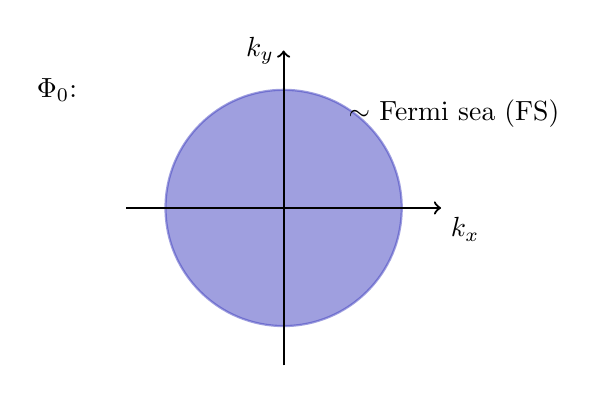
\begin{tikzpicture}[scale = 1]
	
	\coordinate (a) at (2, 2);
	\draw[thick,fill, blue!50!gray,  opacity =0.5] (a) circle (1.5);
	
	\draw[thick, ->] (0,2) to (4,2);
	\draw[thick, ->] (2,0) to (2,4);
	
	\node[anchor = north west] at (4, 2) {$k_x$};	
	
	\node[anchor = east] at (2, 4) {$k_y$};
	
	\node[anchor = east] at (-0.5, 3.5) {$\ket{\Phi_0}$:};
	\node[anchor = west] at (2.7, 3.2) {$\sim$ Fermi sea (FS)};
\end{tikzpicture}
%	\caption{The Fermi sea of $\ket{\Phi_0}$}
	\end{subfigure}	
	\begin{subfigure}{\linewidth}
	\centering
	\begin{tikzpicture}[scale=0.8]
	\begin{axis}[
	ticks=none,
	legend style={at={(1,0.4)}},
	ytick = {1},
	ytick style={draw=none},
	yticklabels = {},
	xtick = {1},
%	xticklabels ={$-\pi$,$\pi$},
	xtick style={draw=none},
	xlabel = \large $k$,
	ylabel = \large $\varepsilon_k$,
	axis lines = center,
	ymin = 0,
	ymax = 1.5,
	xmax = 2,
	xmin = -2,
	%x label style={at={(axis description cs:1,0.1)}, anchor = west},
	%y label style={at={(axis description cs:0.15,1)},rotate=-90,anchor=south},
	%xlabel = $x$,
	%sylabel = {$f(x)$},
	]
	
		
		\addplot[name path = A,domain = -1.57:1.57, samples = 200, very thin, black]{(1-cos(deg(x)))};
		\addplot[domain = -1.7:1.7, samples = 200, thick, red]{(1-cos(deg(x)))};
		\addplot[name path = B, domain = -1.57:1.57] {1+0*x};
		
		\addplot[fill,blue!50!gray, opacity=0.5] fill between[of = A and B];
		
		\draw[thick, black, dashed] (axis cs:-1.57,0) -- node[anchor= north east]{\large $-k_F$}  (axis cs:-1.570,1);
		\draw[thick, black, dashed] (axis cs:1.57,0) -- node[anchor= north west]{\large $k_F$}  (axis cs:1.570,1);
	\end{axis}
\end{tikzpicture}
	\caption{States are filled up to the energy $\ep_F$ at $k = k_F$ according to the Pauli-principle.}
	\end{subfigure}
\end{figure}

i) Consider first $t_2 >t_1$:

\begin{align*} 
&G_0(\lambda_1, t_1, \lambda_2, t_2) \\
 &=-i\theta(t_2-t_1)\ev{c_{k_2,\sigma_2}(t_2)c_{k_1\sigma_1}^\dagger(t_1)}{\Phi_0} \\
&=-i\theta(t_2-t_1)\ev{\e^{i\Ha_0t_2}c_{k_2\sigma_2}\e^{-i\Ha_0t_2}\e^{i\Ha_0t_1}c_{k_1\sigma_1}^\dagger\e^{-i\Ha_0t_1}}{\Phi_0} \\
&= -i\theta(t_2 - t_1) \ev{\e^{i(E_0 + \ep_{k_1}-\ep_{k_2})t_2}c_{k_2\sigma_2}\e^{-i(E_0 + \ep_{k_1})t_2}\e^{i(E_0 + \ep_{k_1})t_1}c_{k_1\sigma_1}^\dagger\e^{-E_0t_1}}{\Phi_0} \\
&= -i\theta(t_2-t_1)\e^{i(\ep_{k_1}-\ep_{k_1})t_2}\e^{-i\ep_{k_1}(t_2-t_1)}\underbrace{\ev{c_{k_2\sigma_2}c_{k_1\sigma_1}^\dagger}{\Phi_0}}_{\delta_{k_1k_2}\delta_{\sigma_1\sigma_2}\theta(\ep_{k_1} - \ep_{k_F})} \\
&= -i\theta(t_2-t_1)\e^{-i\ep_{k_1}(t_2-t_1)}\delta_{k_1k_2}\delta_{\sigma_1\sigma_2}\theta(\ep_{k_1} - \ep_{k_F})
\end{align*}


ii) $t_1>t_2$:

\begin{align*} 
&G_0(\lambda_1, t_1, \lambda_2, t_2) \\
&=-i\theta(t_1-t_2)(-1)\ev{c_{k_1\sigma_1}^\dagger(t_1)c_{k_2,\sigma_2}(t_2)}{\Phi_0} \\
&=i\theta(t_1-t_2)\ev{\e^{i\Ha_0t_1}c_{k_1\sigma_1}^\dagger\e^{-i\Ha_0t_1}\e^{i\Ha_0t_2}c_{k_2\sigma_2}\e^{-i\Ha_0t_2}}{\Phi_0} \\
&= i\theta(t_1-t_2) \ev{\e^{i(E_0 + \ep_{k_1}-\ep_{k_2})t_1}c_{k_1\sigma_1}^\dagger\e^{-i(E_0 - \ep_{k_2})t_1}\e^{i(E_0 - \ep_{k_2})t_2}c_{k_2\sigma_2}\e^{-E_0t_2}}{\Phi_0} \\
&= i\theta(t_1-t_2)\e^{i\ep_{k_1}t_1}\e^{-i\ep_{k_2}t_2}\delta_{k_1k_2}\delta_{\sigma_1\sigma_2}\theta(\ep_{k_F} - \ep_{k_1}) \\
&= i\theta(t_1-t_2)\delta_{k_1k_2}\delta_{\sigma_1\sigma_2}\theta(\ep_{k_F} - \ep_{k_1})\e^{-i\ep_{k_1}(t_2-t_1)}
\end{align*}

Therefore, 
\begin{align}
\label{eq:greens_time_domain}
\begin{split}
G_0(k_1\sigma_1, t_1;k_2\sigma_2, t_2) = &-i\theta(t_2-t_1)\theta(\ep_{k_1} - \ep_{k_F})\delta_{k_1k_2}\delta_{\sigma_1\sigma_2}\e^{-i\ep_{k_1}(t_2-t_1)}\\
&+ i \theta(t_1-t_2)\theta(\ep_{k_F} - \ep_{k_1})\delta_{k_1k_2}\delta_{\sigma_1\sigma_2}\e^{-i\ep_{k_1}(t_2-t_1)}
\end{split}
\end{align}
This is a rather unwieldy expression, so to simplify a bit, we set $t_2-t_1 = t$ and introduce Fourier-transformed $G_0$.

\begin{align*} 
G_0(k_1\sigma_1;k_2\sigma_2;\omega) &= \int_{-\infty}^\infty\dd{t}G_0(k_1\sigma_1;k_2\sigma_2 ; t)\e^{i\omega t} \\
&= -i\theta(\ep_{k_1} - \ep_{k_F})\delta_{k_1k_2}\delta_{\sigma_1\sigma_2}\int_{0}^\infty\dd{t}\e^{-i\ep_{k_1}t}\underbrace{\e^{-\delta t}}_{\delta = 0^+}\e^{i\omega t} \\
&+ i\theta(\ep_{k_F} - \ep_{k_1})\delta_{k_1k_2}\delta_{\sigma_1\sigma_2}\int_{-\infty}^0\dd{t}\e^{-i\ep_{k_1}t}\underbrace{\e^{\delta t}}_{\delta = 0^+}\e^{i\omega t} \\
&= -i\theta(\ep_{k_1} - \ep_{k_F})\delta_{k_1k_2}\delta_{\sigma_1\sigma_2}\int_{0}^\infty \dd{t}\e^{i(\omega -\ep_{k_1} + i\delta)t} \\
& + i\theta(\ep_{k_F} - \ep_{k_1})\delta_{k_1k_2}\delta_{\sigma_1\sigma_2}\int_{-\infty}^0\dd{t}\e^{i(\omega-\ep_{k_1}-i\delta)t} \\
&= \delta_{k_1k_2}\delta_{\sigma_1\sigma_2}\left( \frac{\theta(\ep_{k_1} - \ep_{k_F})}{\omega-\ep_{k_1} + i\delta} + \frac{\theta(\ep_{k_F}-\ep_{k_1})}{\omega - \ep_{k_1} - i\delta} \right)
\end{align*}
\begin{itemize}
	\item The first term in the Green's function involves excitations \underline{above} the Fermi-surface (particles), depicted in \cref{fig:fermi_sea_particle_excitation}.
	\begin{figure}
		\centering
		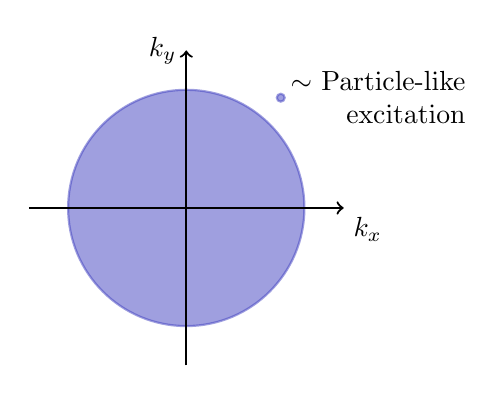
\begin{tikzpicture}[scale = 1]
	
	\coordinate (a) at (2, 2);
	\draw[thick,fill, blue!50!gray,  opacity =0.5] (a) circle (1.5);
	
	\draw[thick, ->] (0,2) to (4,2);
	\draw[thick, ->] (2,0) to (2,4);
	
	\node[anchor = north west] at (4, 2) {$k_x$};	
	
	\node[anchor = east] at (2, 4) {$k_y$};
	
	
	\draw[thick, fill, blue!50!gray, opacity=0.5] (3.2, 3.4) circle (0.05);
%	
%	\node[anchor = east] at (-0.5, 3.5) {$\ket{\Phi_0}$:};
	\node[anchor = west, align = right] at (3.2, 3.4) {$\sim$ Particle-like\\excitation};
\end{tikzpicture}
		\caption{Particle excitation above the Fermi-surface.}
		\label{fig:fermi_sea_particle_excitation}
	\end{figure}
	Particle created first, then destroyed later. Particle moves \underline{forward} in time. This is seen directly from the expression for $G_0$ in the time-domain, \cref{eq:greens_time_domain}, when $t_2 > t_1$ (particle created first at time $t_1$, then destroyed later at time $t_2$).
	\item The second term in the Green's function involves excitations \underline{below} the Fermi-surface (holes), depicted in \cref{fig:fermi_sea_hole_excitation}.
	\begin{figure}
		\centering
		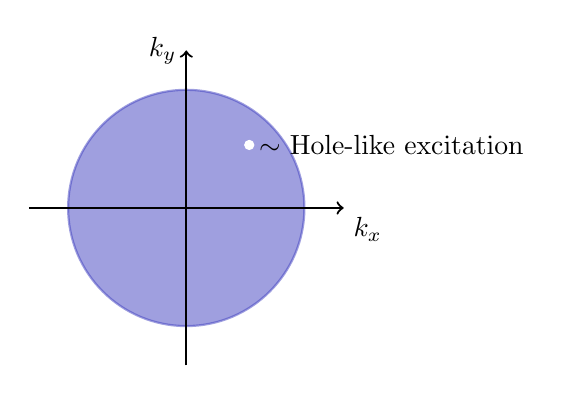
\begin{tikzpicture}[scale = 1]
	
	\coordinate (a) at (2, 2);
	\draw[thick,fill, blue!50!gray,  opacity =0.5] (a) circle (1.5);
	
	\draw[thick, ->] (0,2) to (4,2);
	\draw[thick, ->] (2,0) to (2,4);
	
	\node[anchor = north west] at (4, 2) {$k_x$};	
	
	\node[anchor = east] at (2, 4) {$k_y$};
	
	
	\coordinate (c) at (2.8, 2.8);
	\draw[thick, fill, white] (c) circle (0.05);
%	
%	\node[anchor = east] at (-0.5, 3.5) {$\ket{\Phi_0}$:};
	\node[anchor = west, align = right] at (c) {$\sim$ Hole-like excitation};
\end{tikzpicture}
		\caption{Hole excitation below the Fermi-surface.}
		\label{fig:fermi_sea_hole_excitation}
	\end{figure}
	Particle destroyed first, then created later. Particle moves \underline{backwards} in time. This is again seen directly in \cref{eq:greens_time_domain}.
	\item The part of $G_0$ that moves a particle \underline{forward in time} is often referred to as a \underline{retarded Green's function} $G_0^R$.
	\item The part of $G_0$ that moves a particle \underline{backwards in time} is often referred to as a \underline{advanced Green's function} $G_0^A$.
\end{itemize}


\begin{align} 
G_0^R(k_1, \sigma_1;k_2, \sigma_2;\omega) &= \frac{\theta(\ep_{k_1}-\ep_F)}{\omega_-\ep_{k_1} + i\delta}\delta_{k_1k_2}\delta_{\sigma_1\sigma_2}\\
G_0^A(k_1, \sigma_1;k_2, \sigma_2;\omega) &= \frac{\theta(\ep_F - \ep_{k_1})}{\omega_-\ep_{k_1} - i\delta}\delta_{k_1k_2}\delta_{\sigma_1\sigma_2}
\end{align}
With the understanding that in $G_0$, we must have $k_1 = k_2$; $\sigma_1 = \sigma_2$ and $\ep_{k_1}>\ep_F$ in $G^R$, $\ep_{k_!}<\ep_F$ in $G^A$, we may write
\begin{align} 
G_0^R(k, \omega) &= \frac{1}{\omega -\ep_k + i\delta} \\
G_0^A(k, \omega) &= \frac{1}{\omega -\ep_k -i\delta},
\end{align}
which is summarized by
\begin{align} 
G_0(k, \omega) &= \frac{1}{\omega-\ep_k + i\delta_k},
\end{align}
where $\delta_k = \delta\sign(\ep_k - \ep_F)$.
\begin{tcolorbox}
	Note that the single-particle excitation energies appear as simple poles in the Green's function!
\end{tcolorbox}
To aget a bit more perspective on things, consider $G_0^R (k,\omega)$ a bit further. $G_{0,R}^{-1} = \omega-\ep_k+i\delta$
Imagine that we now introduce $V \ne 0$. What will happen is that the excitation spectrum $\ep_k$ will change, due to the perturbation $G_{0R}^{-1} \rightarrow G_R^{-1}(k,\omega)$.
\begin{equation} 
G_R^{-1}(k,\omega) = \omega -\ep_k -\Sigma(k,\omega),
\end{equation}
$\Sigma(k,\omega) = \Sigma_{\text{Re}}(k,\omega) + i\Sigma_{\text{Im}}(k,\omega)$.
\begin{align*} 
\Sigma_{\text{Re}}: && \text{Real part of } \Sigma \\
\Sigma_{\text{Im}}: && \text{Imaginary part of } \Sigma
\end{align*}
Physicall interpretation og $G_R$: Create a particle in $(k,\sigma)$ at $t=0$. What is the probability amplitude of finding the particle in the same state at $t>0$? \underline{Answer: $G_R$}. $\Sigma(k,\omega)$ is the single particle self-energy.
Note: $G_R^{-1} = G_{0R}^{-1} - \Sigma$
\begin{align*} 
G_R &= \frac{1}{G_{0R}^{-1} - \Sigma} =\frac{G_{0R}}{1-G_{0R}\Sigma} \\
&= G_{0R} + G_{0R}\Sigma G_{0R} + G_{0R}\Sigma G_{0R} \Sigma G_{0R} + \dots
\end{align*}
We can generate a perturbation expansion for $G_R$ by a much simpler perturbation expansion for $\Sigma$!
Define the spectral weight $A_R(k,\omega)$
\begin{equation} 
\label{eq:spectral_function}
A_R(k,\omega) = -\frac{1}{\pi}\Im{G_R(k,\omega)}
\end{equation}
This is the quantity one measures in ARPES 
\begin{equation} 
A_R(k,\omega) = -\frac{1}{\pi}\frac{\Sigma_{\text{Im}}}{(\omega -\ep_k -\Sigma_{\text{Re}})^2-\Sigma_{\text{Im}}^2}
\end{equation}
In the non-interacting case:
$\Sigma_{\text{Im}} = 0, \Sigma_{\text{Im}} = -\delta; \delta = 0^+$
\begin{equation} 
A_{0R}(k, \omega) = -\frac{1}{\pi}\frac{-\delta}{(\omega-\ep_k)^2 + \delta^2} = \delta(\omega -\ep_k),
\end{equation}
which is a Dirac $\delta$-function, shown in \cref{fig:dirac_delta}. Send in photons of different energies and momenta to map out $\ep_k$. 
\begin{figure}
	\begin{subfigure}{0.5\linewidth}
	\centering
	\begin{tikzpicture}[scale=0.8]
	\begin{axis}[
%	ticks=none,
	legend style={at={(1,0.4)}},
	ytick = {1},
	ytick style={draw=none},
	yticklabels = {},
	xtick = {1},
	xticklabels ={\Large $\ep_k$},
%	xtick style={draw=none},
	xlabel = \Large $\omega$,
	ylabel = \Large $A_{0R}$,
	axis lines = center,
%	ymin = 0,
	ymax = 1.5,
%	xmax = 2,
%	xmin = -2,
	x label style={at={(axis description cs:1,0.1)}, anchor = west},
	y label style={at={(axis description cs:0,1)},rotate=0,anchor=west},
	%xlabel = $x$,
	%sylabel = {$f(x)$},
	]
	
		
		\addplot[name path = A,domain = 0:2, samples = 200, blue!50!gray, opacity=0.5, very thick]{0.001/((x-1)^2 + 0.001^2)};
%		\addplot[domain = -1.7:1.7, samples = 200, thick, red]{(1-cos(deg(x)))};
%		\addplot[name path = B, domain = -1.57:1.57] {1+0*x};
		
		\node[anchor= west, align=center] at (axis cs:1,1) {\Large{ $\sim \delta-$function}\\\Large {peak}};
		
%		\draw[thick, black, dashed] (axis cs:-1.57,0) -- node[anchor= north east]{\large $-k_F$}  (axis cs:-1.570,1);
%		\draw[thick, black, dashed] (axis cs:1.57,0) -- node[anchor= north west]{\large $k_F$}  (axis cs:1.570,1);
	\end{axis}
\end{tikzpicture}
	\caption{Non-interacting system.}
	\label{fig:dirac_delta}
	\end{subfigure}
	\begin{subfigure}{0.5\linewidth}
	\centering
	\begin{tikzpicture}[scale=0.8]
	\begin{axis}[
%	ticks=none,
	legend style={at={(1,0.4)}},
	ytick = {1},
	ytick style={draw=none},
	yticklabels = {},
	xtick = {1},
	xticklabels ={\Large $\ep_k + \Sigma_{\text{Re}}$},
%	xtick style={draw=none},
	xlabel = \Large $\omega$,
	ylabel = \Large $A_{R}$,
	axis lines = center,
%	ymin = 0,
	ymax = 9,
%	xmax = 2,
%	xmin = -2,
	x label style={at={(axis description cs:1,0.1)}, anchor = west},
	y label style={at={(axis description cs:0,1)},rotate=0,anchor=west},
	%xlabel = $x$,
	%sylabel = {$f(x)$},
	]
	
		
		\addplot[name path = A,domain = 0:2, samples = 200, black]{0.15/((x-1)^2 + 0.15^2)};
%		\addplot[domain = -1.7:1.7, samples = 200, thick, red]{(1-cos(deg(x)))};
%		\addplot[name path = B, domain = -1.57:1.57] {1+0*x};
		
		\node[anchor= west, align=center] at (axis cs:1.15,3.4) {\Large{$\sim \Sigma_{\text{Im}}$}};
		
		\draw[black, dashed] (axis cs:1,0) --  (axis cs:1,9);
		\draw[very thick, black] (axis cs:1,3.4) --  (axis cs:1.15,3.4);
%		\draw[thick, black, dashed] (axis cs:1.57,0) -- node[anchor= north west]{\large $k_F$}  (axis cs:1.570,1);
	\end{axis}
\end{tikzpicture}
	\caption{Interacting system.}
	\label{fig:lorentzian}
	\end{subfigure}
	\caption{Spectral weights for both interacting and non-interacting system.}
\end{figure}
For $V\ne 0:$ Peak position is shifted, narrow peak is broadened, as shown in \cref{fig:lorentzian}.
From maximum in peak: $\ep_k + \Sigma_{\text{Re}} = \tilde{\ep}_k$. From width of peak: $\Sigma_{\text{Im}}$.
$\Sigma = \Sigma_{\text{Re}} + i\Sigma_{\text{Im}}$. $\Sigma_{\text{Re}}$ and $\Sigma_{\text{Im}}$ are related via the Kramers-Kronig relations
\begin{equation} 
\Sigma_R(k,\omega) = \frac{1}{\pi}\mathcal{P}\int_{-\infty}^\infty\dd{\omega'}\frac{\Sigma_{\text{Im}}(k,\omega')}{\omega'-\omega}.
\end{equation}
Therefore, from width of peak $\rightarrow \Sigma_{\text{Im}}$. From Kramers-Kronig: $\Sigma_{\text{Re}}$. This allows an ARPES experiment to uniquely determine both $\Sigma_{\text{Im}}$ and $\Sigma_{\text{Re}}$ from one measurement, and thus to back out the many-body effect in  $\tilde{\ep}_k$, the quasiparticle excitation spectrum. Note: For Kramers-Kronig to hold, $\Sigma(k,\omega)$ need to be analytic in the upper half-plane when $\omega$ is viewed as a complex variable. Moreover, $\Sigma$ must fall off faster than $\frac{1}{|\omega|}$ when $|\omega| \rightarrow \infty.$ For the perturbations we will consider, this will be the case. 
\begin{tcolorbox}
	Our goal will therefore be to compute $\Sigma$ in many-body perturbation theory.
\end{tcolorbox}
Before we go into this, it will be turn out to be necessary to also consider bosonic Green's functions, and we start with the non-interacting case
\subsection{Bosons} % Lecture notes week 7

\begin{align*} 
D(q, t-t') &= -i\ev{\tilde{T}[\hat{A}_q(t)\hat{A}_q^\dagger(t')]}{\Psi(0)} \\
&= -i\frac{\ev{\tilde{T}[\hat{A}_q(t)\hat{A}_q^\dagger(t')S(\infty, -\infty)]}{\Phi_0}}{\ev{S(\infty, -\infty)}{\Phi_0}}.
\end{align*}
$\ket{\Phi_0}$: Unperturbed ground state of bosonic system. 
\begin{equation} 
\label{eq:non_int_greens_boson}
D_0(q, t-t') = -i\ev{\tilde{T}[\hat{A}_q(t)\hat{A}_q^\dagger(t')]}{\Phi_0}.
\end{equation}
Retarded boson-propagator: $t'<t$. Advanced boson-propagator: $t'>t$. At $T = 0$, the lowest energy state is occupied by all bosons (material particles), or there are no bosons present at all (phonons, magnons).
Let us focus in the following focus on \underline{phonons}.
\begin{align*} 
A_q &= a_q + a_{-q}^\dagger \\
A_q(t) &= \e^{i\Ha_0 t}A_q\e^{-i\Ha_0t} \\
\Ha_0 &= \sum_{q, \lambda }\omega_{q, \lambda}a_{q,\lambda}^\dagger a_{q,\lambda} \\
\Ha_0\ket{\Phi_0} &= 0 = E_0\ket{\Phi_0}, E_0 = 0
\end{align*}
$t'=0$, since $D_0$ will only be a function of $t-t'$ anyway. This is no loss of generality.

\textbf{$t>0$}:
\begin{align} 
\begin{split} 
D_0(q, \lambda, t) &= -i\theta(t)\ev{\e^{i\Ha_0 t}A_{q\lambda}\e^{-i\Ha_0t}A_{q\lambda}^\dagger}{\Phi_0} \\
&= -i\theta(t)\ev{A_{q\lambda}A_{q\lambda}^\dagger}{\Phi_0}\e^{-i\omega_{q,\lambda}t}\\
&= -i\theta(t)\e^{-i\omega_{q, \lambda}t}
\end{split}
\end{align}

\textbf{$t<0$}:
\begin{align} 
\begin{split} 
D_0(q, \lambda, t) &= -i\theta(-t)\ev{A_{q\lambda}^\dagger\e^{i\Ha_0 t}A_{q\lambda}\e^{-i\Ha_0t}}{\Phi_0} \\
&= -i\theta(-t)\ev{A_{q\lambda}^\dagger A_{q\lambda}}{\Phi_0}\e^{i\omega_{q,\lambda}t}\\
&= -i\theta(-t)\e^{i\omega_{q, \lambda}t}.
\end{split}
\end{align}

In total we have
\begin{equation} 
D_0(q, \lambda, t) = -\theta(t)\e^{-i\omega_{q, \lambda}t} -i\theta(-i)\e^{i\omega_{q,\lambda}t}.
\end{equation}
Note the sign change in the phase factor due to $A_q = a_q+ a_{-q}^\dagger$.
As for the fermionic case, let us Fourier-transform this, using shorthand notation $q = (q, \lambda)$.

\begin{align} 
\begin{split} 
D_0(q, \omega) &= \int_{-\infty}^\infty\dd{t}\e^{i\omega t}D_0(q, t) \\
&= -i\int_{0}^{\infty}\dd{t}\e^{i(\omega-\omega_{q} + i\delta)t} -i \int_{-\infty}^{0}\dd{t}\e^{i(\omega + \omega_{q} -i\delta)t} \\
&= \frac{1}{\omega -\omega_q + i\delta} - \frac{1}{\omega + \omega_q -i\delta} \\
&= \frac{2\omega_q}{\omega^2-\omega_q^2 + i\eta}.
\end{split}
\end{align}
Here, it does not make sense to consider retarded and advanced parts as for the fermions, since $A_q = a_q + a_{-q}^\dagger$
\begin{equation} 
D_0^{-1} = \frac{\omega^2 - \omega_q^2}{2\omega_q} + i\eta
\end{equation}
Imagine now that we turn on interactions (between phonons and electrons, for example)

\begin{tcolorbox}
\begin{equation} 
D_0^{-1} \rightarrow D^{-1} = D_{0}^{-1} - \Pi
\end{equation}
\end{tcolorbox}
$\Pi:$ Phonon self-energy.
\begin{align*} 
D &= \frac{1}{D_0^{-1} - \Pi} = \frac{D_0}{1-\Pi D_0} \\
&= D_0  + D_0\Pi D_0 + D_0 \Pi D_0\Pi D_0 + \dots
\end{align*}
Again; Perturbation series for $D$ by much simpler perturbation series for $\Pi$!

The equations
\begin{align} 
G_R^{-1} &= G_{0R}^{-1} - \Sigma \\
D^{-1} &= D_{0}^{-1} - \Pi
\end{align}
are usually referred to as the \textbf{Dyson's equations} for single-particle Green's functions. The physicall interpretations for $G$ and $D$ are the same (but of course applies to two different sorts of particles.)
In the following, we will consider electron- phonon coupling as a perturbation. The phonons will lead to a $\Sigma$, and the electrons in turn will lead to a $\Pi$.

\section[Single particle Green's function]{Perturbation theory for the single-particle Green's function}
Denote this Green's function by $G(\lambda, t-t')$. We have previously argued that in the presence of interactions it may be expressed as follows
\begin{equation} 
G^{-1} = G_0^{-1} - \Sigma
\end{equation}
where $G_0$ is the single-particle Green's function in the non-interacting case, and $\Sigma$ is the self-energy. Thus, our perturbation theory for $G$ may be found by a perturbation expansion for $\Sigma$, which we may hope is easier to compute than a perturbation theory for $G$ directly. The basic mathematical expression for $G$ is, starting in the Heisenberg-picture
\begin{equation} 
G(\lambda, t-t') = -i\ev{\tilde{T}[\hat{c}_\lambda(t)\hat{c}_\lambda^\dagger(t')]}{\psi(0)}
\end{equation}
where $\ket{\psi(0)}$ are exact eigenstates and 
\begin{equation} 
\hat{c}_\lambda(t) = \e^{i\Ha t}c_\lambda\e^{-i\Ha t}.
\end{equation}
Translated into interaction picture, we have
\begin{equation} 
G(\lambda, t-t') = -i\frac{\ev{\tilde{T}[{c}_{\lambda}(t){c}_{\lambda}^\dagger(t')S(\infty, -\infty)]}{\Phi_0}}{\ev{S(\infty, -\infty)}{\Phi_0}},
\end{equation}
where $S$ is the $S$-matrix,
\begin{equation} 
c_\lambda(t) = \e^{i\Ha_0 t}c_\lambda\e^{-i\Ha_0 t},
\end{equation}
and $\ket{\Phi_0}$  is the eigenstate of $\Ha_0$, assumed to be known to us. 
Both of these expressions are formally exact, while the second one allows a systematic expansion in powers of $V(t)$, where
\begin{equation} 
V(t) = \e^{i\Ha_0 t}V\e^{-i\Ha_0 t}
\end{equation}
and $\Ha = \Ha_0 + V$.
For $S(\infty, -\infty)$, we have (remember \cref{eq:s_matrix})
\begin{equation} 
S(t, t') =  \sum_{n=0}^{\infty}\frac{(-i)^n}{n!}\int_{t'}^{t}\dd{t_1}\cdots\int_{t'}^{t}\dd{t_n}\tilde{T}[V(t_1)\cdots V(t_n)]
\end{equation}
where the $n=0$-term is 1. 
In these notes, we will focus on $V$ taken to be the electron-phonon coupling. Another obvious choice would be the Coulomb-interaction. 
\begin{equation}
\label{eq:el_ph}
V =\sum_{k,q, \sigma, \lambda}g_{q\lambda}A_{q\lambda} c_{k+q,\sigma}^\dagger c_{k,\sigma},
\end{equation}
$A_{q\lambda} = a_{-q,\lambda}^\dagger + a_{q\lambda}$.

\begin{align*} 
V(t) &= \e^{i\Ha_0 t}V\e^{-i\Ha_0 t} \\
&=  \sum_{k,q, \sigma, \lambda}g_{q\lambda}\e^{i\Ha_0 t}A_{q\lambda} c_{k+q,\sigma}^\dagger c_{k,\sigma}\e^{-i\Ha_0 t} \\
&= \sum_{k,q, \sigma, \lambda}g_{q\lambda}\left(\vphantom{c_{k+q,\sigma}^\dagger}\e^{i\Ha_0 t}A_{q\lambda}\e^{-i\Ha_0 t}\right)\left( \e^{i\Ha_0 t}c_{k+q,\sigma}^\dagger\e^{-i\Ha_0 t}\right)\left( \vphantom{c_{k+q,\sigma}^\dagger} \e^{i\Ha_0 t}c_{k,\sigma}\e^{-i\Ha_0 t}\right)
\end{align*}
\begin{tcolorbox}
	\begin{equation}
	\label{eq:el_ph_time}
		V(t) = \sum_{k, q, \sigma, \lambda}g_{q\lambda}A_{q\lambda}(t) c_{k+q,\sigma}^\dagger(t) c_{k,\sigma}(t)
	\end{equation}
\end{tcolorbox}
Compare $V(t)$ in \cref{eq:el_ph_time} to $V$ in \cref{eq:el_ph}. All time-dependence of operators is in the interaction picture. $V(t)$ is the perturbation we will use in $ S(\infty, -\infty) $ and thus $G(\lambda, t-t')$. The expectation values we will have to compute will then consist of a product of $ (c^\dagger, c)$-operators multiplied by a product of $ A$-operators. 
Each $ V $ will give a factor $ Ac^\dagger c $. Thus, $n$ factors of $V$ will give
\begin{equation} 
\left.\begin{array}{cc}
n+1 & c^\dagger \text{-factors} \\
n+1 & c \text{-factors} \\
n & A\text{ -factors}
\end{array}\right\} \text{ in } G
\end{equation}
The extra 1 in $n+1$ comes from $c_\lambda^\dagger(t'), c_\lambda(t)$  in the definition of $G$. Now, we factorize $\ket{\Phi_0}$ in a \textbf{boson-part} and a \textbf{fermion-part}. 
\begin{equation} 
\left.\begin{array}{cc}
\text{ Boson-part: } & \ket{\Phi_0}_B \\
\text{ Fermion-part: } & \ket{\Phi_0}_F
\end{array}\right\} \implies \ket{\Phi_0} = \ket{\Phi_0}_B \otimes \ket{\Phi_0}_F.
\end{equation}
\begin{align} 
\begin{split} 
G(\lambda, t-t') &= \frac{-i}{\ev{S(\infty, -\infty)}{\Phi_0}}\sum_{n=0}^{\infty}\frac{(-i)^n}{n!}\int_{-\infty}^{\infty}\dd{t_1}\dots  \int_{-\infty}^{\infty}\dd{t_n} \\
& \cdot \ev{\tilde{T}[c_\lambda(t)c_\lambda^\dagger(t')V(t_1)\dots V(t_n)]}{\Phi_0}.
\end{split}
\end{align}
$[\ \cdot\ ]$: A product of $n+1$ $ c^\dagger, c $-operators and $n$ $A(t_i)$-operators. The expectation value of the fermion-operators are taken in $\ket{\Phi_0}_F$, while the expectation value of the boson-operators are taken in $\ket{\Phi_0}_B$. The expectation value may thus be written
\begin{align*} 
&{}_B\ev{\tilde{T}[A_{q_1}(t_1)\dots A_{q_n}(t_n)]}{\Phi_0}_B\\
& \cdot {}_F\ev{\tilde{T}[c_\lambda(t)c_\lambda^\dagger(t') c_{k_1+q, \sigma_1}^\dagger(t_1) c_{k_1\sigma_1}(t_1)\dots c_{k_n+q, \sigma_n}^\dagger(t_n) c_{k_n\sigma_n}(t_n)]}{\Phi_0}_F
\end{align*}
\textbf{NB!} Be careful with the ordering of operators! We see that as $n$ increases, the number of operators rapidly becomes sizeable, particularly in the fermionic part. One thing we immediately note, is that for these expectation values to be non-zero, we must have an even number of $A$-operators. Thus, for the electron-phonon coupling, only even powers of $ V $ contribute to the perturbation-series for $G$. (This is not the case if $V$ were taken to be the Coulomb-interaction, which contains $c^\dagger c^\dagger c c$ and no boson-operators.)
The lowest order term we need to consider, is therefore $n=2$, which contains 2 $A$-operators and 6 fermion-operators. For $n=2$, the boson-part is easy. Recall that 
\begin{align*} 
D_0(q, t) = -i {}_B&\ev{\tilde{T}[A_q(t)A_q(0)]}{\Phi_0}_B \\
\implies& \\
{}_B&\ev{\tilde{T}[A_q(t_1)A_q(t_2)]}{\Phi_0}_0 = iD_0(q, t_1-t_2),
\end{align*}
the free phonon Green's function we already computed. 
Next, we need to deal with the expectation value of a string of a fairly large number of fermion-operators (6 of them for $n=2$. 3$c^\dagger $ and $3 c$).
To do this, we use a theorem which we give here without proof. 
\begin{tcolorbox}[title= Wicks theorem]

To compute the $\ket{\Phi_0}_F$-expectation value of a product of equally many $c^\dagger$ and $c$-operators, we pair in all possible ways and compute the expectation value as products of expectation values of one $c^\dagger$ and one $c$. 
\end{tcolorbox}
\textbf{NB!} When pairing up non-adjacent $c^\dagger $ and $c$, use anti-commutation relations to bring them side by side to compute an expectation value.
Suppose we have a product of $N$ creation operators and $N$ destruction operators (bosonic of fermionic). The number of terms we then get by applying Wick's theorem is $N!$ Thus for $n=2$ with 3 $c^\dagger$ and 3 $c$, the number of terms is $3! =6$. 
To fourth order, the number of bosonic terms will be $6\cdot2! = 12 $ (since when expanding $A_q = a_{-q}^\dagger + a_q$ to fourth order there are 6 terms with 2 $a^\dagger$ and 2 $a$, and Wick's theorem applied to each of them gives another factor 2. The number of fermionic terms is given by $N= n+1 = 5 \rightarrow 5! =120. $ Altogether $12\cdot 120 = 1440$ terms. This rapidly gets out of hand, if we don't think a little and organize the calculations in a smart way. 
Recall the definitions of the non-interacting Green's functions of \cref{eq:non_int_greens_boson,eq:non_int_greens_fermion};
\begin{align} 
D_0(q_1, t_1-t_2)\delta_{q_1, q_2} &= -i\ev{\tilde{T}[A_{q_1}(t)A_{q_2}^\dagger(t')]}{\Phi_0}_B\\[2ex]
G_0(k_1, t_1-t_2)\delta_{k_1k_2}\delta_{\sigma_1\sigma_2} &= -i\ev{\tilde{T}[c_{k_1\sigma_1}^\dagger(t_1)c_{k_2\sigma_2}(t_2)]}{\Phi_0}_F
\end{align}
We will give these the following pictorial representation:
\begin{equation}
D_0(q_1, t_1-t_2): \quad 
\begin{tikzpicture}
\begin{feynman}
\vertex [small, dot](a) {};
\vertex [small, dot, right = 2cm of a] (b) {};
\diagram*{(a) [dot] --[boson, edge label=$q_1$] (b) [dot]};
\node[anchor = east] at (a) {$t_1$};
\node[anchor = west] at (b) {$t_2$};	
\end{feynman}
\end{tikzpicture}
\end{equation}
\begin{equation} 
G_0(k_1, t_1-t_2): \quad 
\begin{tikzpicture}
\begin{feynman}
\vertex [small, dot](a) {};
\vertex [small, dot, right = 2cm of a] (b) {};
\diagram*{(a) [dot] --[fermion] (b) [dot]};
\node[anchor = east] at (a) {$t_1$};
\node[anchor = west] at (b) {$t_2$};	
\end{feynman}
\end{tikzpicture}
\end{equation}
These will turn out to be very helpful later on. 

\underline{Start with $\ev{S(\infty, -\infty)}{\Phi_0}$}:
\begin{align*} 
&\ev{S(\infty, -\infty)}{\Phi_0} \\
&= 1 + \frac{(-i)^2}{2!}\int_{-\infty}^\infty\dd{t_1}\int_{-\infty}^\infty\dd{t_2}\ev{\tilde{T}[V(t_1)V(t_2)]}{\Phi_0} + \mathcal{O}(V^4)
\end{align*}
Consider now in detail the second term

\begin{align*} 
\frac{(-i)^2}{2!}&\int_{-\infty}^\infty\dd{t_1}\int_{-\infty}^\infty\dd{t_2}\sum_{k_1, q_1, \sigma_1}\sum_{k_2, q_2, \sigma_2}g_{g_1}g_{q_2}\\
&\cdot{}_B\ev{\tilde{T}[A_{q_1}(t_1)\underbrace{A_{q_2}(t_2)}_{=A_{-q_2}^\dagger(t_2)}]}{\Phi_0}_B \\
&\cdot {}_F\ev{\tilde{T}[c_{k_1+q_1, \sigma_1}^\dagger(t_1) c_{k_1\sigma_1}(t_1) c_{k_2+q_2, \sigma_2}^\dagger(t_2) c_{k_2\sigma_2}(t_2)]}{\Phi_0}_F
\end{align*}
The bosonic expectation value $= iD_0(q_1, t_1-t_2)\delta_{q_1, -q_2}$. In the fermionic part, use Wick's theorem. There are 2 ways to pair the $c^\dagger$'s with the $c$'s.
\begin{enumerate}[i)]
	\item \begin{equation}
		\wick{\c1 c_{k_1+q_1, \sigma_1}^\dagger \c1 c_{k_1\sigma_1} \c2 c_{k_2+q_2, \sigma_2}^\dagger \c2 c_{k_2\sigma_2}}
	\end{equation}
	\item \begin{equation}
	\wick{\c1 c_{k_1+q_1, \sigma_1}^\dagger \c2 c_{k_1\sigma_1} \c2 c_{k_2+q_2, \sigma_2}^\dagger \c1 c_{k_2\sigma_2}}
	\end{equation}
\end{enumerate}
with the corresponding equations
\begin{enumerate}[i)]
	\item \begin{align}
	\begin{split} 
	(+i)&G_0(k_1+q_1, t_1-t_1)\delta_{k_1+q_1,k_1}\cdot(-1)\\
	\cdot(+i)&G_0(k_2+q_2, t_2-t_2)\delta_{k_2+q_2,k_2}\cdot(-1)
	\end{split}	
	\end{align}
	
	\item 
	\begin{align}
	\begin{split} 
	(+i)&G_0(k_1+q_1, t_2-t_1)\delta_{k_1+q_1,k_2}\delta_{\sigma_1\sigma_2}\cdot(-1)^3\\
	\cdot(+i)&G_0(k_2+q_2, t_1-t_2)\delta_{k_2+q_2,k_1}\delta_{\sigma_1\sigma_2}\cdot(-1)
	\end{split}	
	\end{align}
\end{enumerate}
In i), note that the $\delta$-functions in $k$ from the fermionic part forces $q_1 =0, q_2 = 0$.
Multiplying all the factors of i):
\begin{center}
\begin{tikzpicture}
	\begin{feynman}[large]
	\vertex [small, dot] (a) {};
	\vertex [small, dot, right = 3cm of a] (b) {};
	\diagram*{
	a --[anti fermion,loop, min distance=3cm] a -- [boson, edge label'=$q_1$] (b) -- [anti fermion,loop, min distance=3cm] b,	
};
	\node[anchor = east] at ($(a)+(-0.1,0)$) {$g_{-q_1}$};
	\node[anchor = west] at ($(b)+(0.1,0)$)  {$g_{q_1}$};
	\node[anchor = north] at ($(a)+(-0.1,-0.1)$) {$t_1$};
	\node[anchor = north] at ($(b)+(0.1,-0.1)$)  {$t_2$};	
	\end{feynman}
\end{tikzpicture}
\end{center}
But $q_1=q_2 = 0$. Since $g_q =0$ when $q=0$, this contribution to $S$ vanishes.
Consider next ii), which has the following representation:
\begin{center}
	\begin{tikzpicture}
		\begin{feynman}[large]
		\vertex [small, dot] (a) {};
		\vertex [small, dot, right = 3cm of a] (b) {};
		\diagram*{a -- [quarter right, fermion, edge label'={$k_1 + q_1, \sigma_1$}] (b) -- [quarter right, fermion, edge label'={$k_1, \sigma_1$}] a -- [boson, edge label'=$q_1$] (b),};
		
		\node[anchor = east] at ($(a)+(-0.1,0)$) {$g_{-q_1}$};
		\node[anchor = west] at ($(b)+(0.1,0)$)  {$g_{q_1}$};
		\node[anchor = north] at ($(a)+(-0.1,-0.1)$) {$t_1$};
		\node[anchor = north] at ($(b)+(0.1,-0.1)$)  {$t_2$};	
		\end{feynman}
	\end{tikzpicture}
\end{center}
Here, $q_1$ is not restricted to zero, so this contribution is nonzero. We must integrate over $t_1, t_2$, sum over $k_1, q_1, \sigma_1$.
Note $g_{q_1}g_{-q_1} = g_{q_1}g_{q_1}^* = |g_{q_1}|^2$. So to $\mathcal{O}(V^2)$, we have 
\begin{equation} 
\ev{S}{\Phi_0} = 1 +
\begin{gathered}
\feynmandiagram[scale = 2, transform shape][large, horizontal = a to b]{a -- [quarter right, fermion] b -- [quarter right, fermion] a -- [boson] b,};
\end{gathered} 
\end{equation}
The first term is simply the normalization of $\ket{\Phi_0}$. The second contribution is a quantum fluctuation effect in $\ket{\Phi_0}$ due to the presence of phonons. These phonons ``disturb'' the inert state $\ket{\Phi_0}$. This is often called a vacuum-fluctuation. and is a quantum fluctuation effect, which is present even when the system is left all by itself. Note that this contribution enters into the denominator of the Green's function we are in the process of computing. 

Consider next the numerator in $G$. The only difference between the numerator and $\ev{S(\infty, -\infty)}{\Phi_0}$ is the extra $c_{ k\sigma}(t)\cd_{ k\sigma}(t')$. The bosonic part is therefore\ exactly as in  $\ev{S(\infty, -\infty)}{\Phi_0}$, but the fermionic part now have 3 $\cd$'s and 3 $c$'s, instead of 2 $\cd$'s and 2 $c$'s.
We therefore consider only this fermionic expectation value, remembering that the result must be multiplied with\begin{equation} 
iD_0(q_1, t_1-t_2)\delta_{q_1, -q_2}g_{q_1}g_{q_2}. 
\end{equation}
The fermionic expectation value is
\begin{equation} 
{}_F\ev{\tilde{T}[c_{k\sigma}(t)c_{k\sigma}^\dagger(t') c_{k_1+q_1, \sigma_1}^\dagger(t_1) c_{k_1\sigma_1}(t_1) c_{k_2+q_2, \sigma_2}^\dagger(t_2) c_{k_2\sigma_2}(t_2)]}{\Phi_0}_F.
\end{equation}
Using Wicks theorem, the terms are
% c\cd \cd_1 c_1 \cd_2 c_2
\begin{enumerate}[1)]
	\item 
	\begin{equation} 
	\wick{\c c_{k\sigma} \c c_{k\sigma}^\dagger \c c_{k_1+q_1, \sigma_1}^\dagger \c c_{k_1\sigma_1} \c c_{k_2+q_2, \sigma_2}^\dagger \c c_{k_2\sigma_2}}
	\end{equation}
	$\implies \delta_{k_1 + q_1, k_1}\delta_{k_2 + q_2, k_2}\delta_{\sigma_1\sigma_2} \implies q_1=q_2 = 0 \implies \underline{1) = 0}.$
	\item
	\begin{equation} 
	\wick{\c1 c_{k\sigma} \c2 c_{k\sigma}^\dagger \c1 c_{k_1+q_1, \sigma_1}^\dagger \c2 c_{k_1\sigma_1} \c c_{k_2+q_2, \sigma_2}^\dagger \c c_{k_2\sigma_2}}
	\end{equation}
	$\implies \delta_{k, k_1+q_1}\delta_{\sigma, \sigma_1}\delta_{k, k_1}\delta_{k_2 + q_2, k_2} \implies q_2 = 0 \implies \underline{2) = 0}$.\todo{I think there is an error in the notes here for both 2) and 3) in the delta-functions, but the conclusions of zero contribution remains.}
	\item 
	\begin{equation} 
	\wick{\c1 c_{k\sigma} \c2 c_{k\sigma}^\dagger \c c_{k_1+q_1, \sigma_1}^\dagger \c c_{k_1\sigma_1} \c1 c_{k_2+q_2, \sigma_2}^\dagger \c2 c_{k_2\sigma_2}}
	\end{equation}
	$\implies \delta_{k, k_2 +q_2}\delta_{\sigma, \sigma_2}\delta_{k, k_2}\delta_{k_1+q_1, k_1} \implies q_1 = 0 \implies \underline{3) = 0}$.
	\item
	\begin{equation} 
	\wick{\c c_{k\sigma} \c c_{k\sigma}^\dagger \c1 c_{k_1+q_1, \sigma_1}^\dagger \c2 c_{k_1\sigma_1} \c2 c_{k_2+q_2, \sigma_2}^\dagger \c1 c_{k_2\sigma_2}}
	\end{equation}
	\begin{align*} 
	=iG_0(k, t-t')&(-i)G_0(k_1+q_1, t_2-t_1)\delta_{k_1+q_1, k_2}\delta_{\sigma_1, \sigma_2} \\
	\cdot&(+i)G_0(k_1, t_1-t_2)\delta_{k_2+q_2, k_1}\delta_{\sigma_1, \sigma_2}
	\end{align*}
	Let us give a pictorial representation of this:
	\begin{center}
		\begin{tikzpicture}
		\begin{feynman}[large]
		\vertex [small, dot] (a) {};
		\vertex [small, dot, right = 3cm of a] (b) {};
		\vertex [small, dot, above = 1.5cm of a] (c) {};
		\vertex [small, dot, right = 3cm of c] (d) {};
		\diagram*{a -- [quarter right, fermion, edge label'={$k_1 + q_1, \sigma_1$}] (b) -- [quarter right, fermion, edge label'={$k_1, \sigma_1$}] a -- [boson, edge label'=$q_1$] (b),
		(c) -- [fermion, edge label = {$k, \sigma$}] (d)};
		
		\node[anchor = east] at ($(a)+(-0.1,0)$) {$g_{-q_1}$};
		\node[anchor = west] at ($(b)+(0.1,0)$)  {$g_{q_1}$};
		\node[anchor = north] at ($(a)+(-0.1,-0.1)$) {$t_1$};
		\node[anchor = north] at ($(b)+(0.1,-0.1)$)  {$t_2$};
		\node[anchor = north] at ($(c)+(-0.1,-0.1)$) {$t'$};
		\node[anchor = north] at ($(d)+(0.1,-0.1)$)  {$t$};
		\end{feynman}
		\end{tikzpicture}
	\end{center}
	This is a disconnected diagram. The interpretation of this is that the electron is disturbed by a quantum fluctuation in $\ket{\Phi_0}$, namely a vacuum-fluctuation. This vacuum-fluctuation is present even if we do not try to inject and extract an electron into the system. This is why the diagram comes out disconnected.
	\item 
	\begin{equation} 
	\wick{\c1 c_{k\sigma} \c2 c_{k\sigma}^\dagger \c1 c_{k_1+q_1, \sigma_1}^\dagger \c3 c_{k_1\sigma_1} \c3 c_{k_2+q_2, \sigma_2}^\dagger \c2 c_{k_2\sigma_2}}
	\end{equation}
	\begin{align*} 
	=(+i)&G_0(k, t-t_1)\delta_{k, k_1+q_1}\delta_{\sigma, \sigma_1}\\(+i)&G_0(k, t_2-t')\delta_{k,k_2}\delta_{\sigma, \sigma_2}\\
	(+i)&G_0(k_1, t_1-t_2)\delta_{k_1, k_2 + q_2}\delta_{\sigma_1, \sigma_2}(-1)^3
	\end{align*}
	We may give the following pictorial representation of this:
		\begin{center}
		\begin{tikzpicture}
		\begin{feynman}[large]
		\vertex [small, dot] (a) {};
		\vertex [small, dot, right = 3cm of a] (b) {};
		\vertex [small, dot, right = 3cm of b] (c) {};
		\vertex [small, dot, right = 3cm of c] (d) {};
		%		\vertex [small, dot, above = 1.5cm of a] (c) {};
		%		\vertex [small, dot, right = 3cm of c] (d) {};
		\diagram*{(a) -- [fermion, edge label={$k,\sigma$}] (b) -- [out=70,in=110, boson, edge label={$k-k_1$}] (c) -- [anti fermion, edge label={$k_1, \sigma$}] (b),
			(c) -- [fermion, edge label ={$k,\sigma$}] (d)
		};
		
		\node[anchor = east] at ($(b)+(-0.0,+0.2)$) {$g_{-q_1}$};
		\node[anchor = west] at ($(c)+(0.0,+0.2)$)  {$g_{q_1}$};
		\node[anchor = north] at ($(a)+(-0.1,-0.1)$) {$t'$};
		\node[anchor = north] at ($(b)+(0.1,-0.1)$)  {$t_2$};
		\node[anchor = north] at ($(c)+(-0.1,-0.1)$) {$t_1$};
		\node[anchor = north] at ($(d)+(-0.1,-0.1)$) {$t$};
		\end{feynman}
		\end{tikzpicture}
	\end{center}

	This is a connected diagram. The Green's function of the electron is disturbed by a quantum fluctuation, but in this case the quantum fluctuation is a direct result of injecting the electron into the system. 
	\item
	\begin{equation} 
	\wick{\c1 c_{k\sigma} \c2 c_{k\sigma}^\dagger \c3 c_{k_1+q_1, \sigma_1}^\dagger \c2 c_{k_1\sigma_1} \c1 c_{k_2+q_2, \sigma_2}^\dagger \c3 c_{k_2\sigma_2}}
	\end{equation}
	\begin{align*} 
	=(+i)&G_0(k, t-t_2)\delta_{k, k_2+q_2}\delta_{\sigma, \sigma_2}\\(-i)&G_0(k, t_1-t')\delta_{k,k_1+q_1}\delta_{\sigma, \sigma_1}\\
	(-i)&G_0(k_1 + q_1, t_2-t_1)\delta_{k_1 + q_1, k_2}\delta_{\sigma_1, \sigma_2}(-1)^4
	\end{align*}
	We may give the following pictorial description of this:
			\begin{center}
		\begin{tikzpicture}
		\begin{feynman}[large]
		\vertex [small, dot] (a) {};
		\vertex [small, dot, right = 3cm of a] (b) {};
		\vertex [small, dot, right = 3cm of b] (c) {};
		\vertex [small, dot, right = 3cm of c] (d) {};
		%		\vertex [small, dot, above = 1.5cm of a] (c) {};
		%		\vertex [small, dot, right = 3cm of c] (d) {};
		\diagram*{(a) -- [fermion, edge label={$k,\sigma$}] (b) -- [out=70,in=110, boson, edge label={$q_1$}] (c) -- [anti fermion, edge label={$k_1 + q_1, \sigma$}] (b),
			(c) -- [fermion, edge label ={$k,\sigma$}] (d)
		};
		
		\node[anchor = east] at ($(b)+(-0.0,+0.2)$) {$g_{-q_1}$};
		\node[anchor = west] at ($(c)+(0.0,+0.2)$)  {$g_{q_1}$};
		\node[anchor = north] at ($(a)+(-0.1,-0.1)$) {$t'$};
		\node[anchor = north] at ($(b)+(0.1,-0.1)$)  {$t_1$};
		\node[anchor = north] at ($(c)+(-0.1,-0.1)$) {$t_2$};
		\node[anchor = north] at ($(d)+(-0.1,-0.1)$) {$t$};
		\end{feynman}
		\end{tikzpicture}
	\end{center}
	Same as 5).
\end{enumerate}
Thus, we get to second order in $g$:
\begin{align*}
	G(k, t-t') &= -i\left\{
	\begin{gathered}
	\feynmandiagram[scale = 1, transform shape][horizontal = a to b]{a --[fermion] b};
	\end{gathered}
	+ 
	\begin{gathered}
	\begin{tikzpicture}
	\begin{feynman}[large]
	\vertex[small,dot] (a) {};
	\vertex [small, dot, right = of a] (b) {};
	\vertex [above = 0.5cm of a] (c) {};
	\vertex [above = 0.5cm of b] (d) {};
	\diagram*{a -- [quarter right, fermion] (b) -- [quarter right, fermion] a -- [boson] (b),
		(c) -- [fermion] (d)};
	\end{feynman}
	\end{tikzpicture}
	\end{gathered}\cdot(-i)^3(-1)
	\right.\\
	&\left. + 2(-i)^3(-1)\feynmandiagram[large][horizontal = a to d]{a--[fermion] b --[fermion] c -- [fermion] d, b--[half left, boson] c};
	+\dots \right\}\frac{1}{1 + \begin{gathered}
		\feynmandiagram[scale = 1, transform shape][large, horizontal = a to b]{a -- [quarter right, fermion] b -- [quarter right, fermion] a -- [boson] b,};
		\end{gathered}(+i)^2(-1)}
\end{align*}
\textbf{Schematically;} to second order in $g$:
\begin{align*}
	G = &\begin{gathered}
	\feynmandiagram[scale = 1, transform shape][horizontal = a to b]{a --[fermion] b};
	\end{gathered}\times \frac{\left(1 +
		\begin{gathered}
		\feynmandiagram[scale = 1, transform shape][large, horizontal = a to b]{a -- [quarter right, fermion] b -- [quarter right, fermion] a -- [boson] b,};
		\end{gathered} + \dots \right)}{1 +
		\begin{gathered}
		\feynmandiagram[scale = 1, transform shape][large, horizontal = a to b]{a -- [quarter right, fermion] b -- [quarter right, fermion] a -- [boson] b,};
		\end{gathered}} \\
	&+ \feynmandiagram[large][horizontal = a to d]{a--[fermion] b --[fermion] c -- [fermion] d, b--[half left, boson] c}; + \dots
\end{align*}
Disconnected diagrams cancel out. This will happen, order by order in $g$, to all orders. 
\begin{tcolorbox}[center, width =0.6\textwidth]
	$G$ is the sum of connected diagrams. 
\end{tcolorbox}
Thus, we are computing corrections to $G_0$ which come about as a direct result of quantum fluctuations that arise \textbf{because} we injected an electron into the system. The vacuum fluctuations cancel out. 
Imagine now that we compute corrections to  higher order in $g$, $g^4, g^6, \dots $ etc.
Schematically, we find 
\begin{align*}
G &=  \underset{g^0}{\begin{gathered}
\feynmandiagram[scale = 1, transform shape][horizontal = a to b]{a --[fermion] b};
\end{gathered}}
 + \underset{g^2}{\begin{gathered}
 \feynmandiagram[large][horizontal = a to d]{a--[fermion] b --[fermion] c -- [fermion] d, b--[half left, boson] c};
\end{gathered}} + \underset{g^4}{\begin{gathered}
\feynmandiagram[large][horizontal = a to f]{a--[fermion] b --[fermion] c -- [fermion] d --[fermion] e --[fermion] f, b--[half left, boson] c, d--[half left, boson] e};
\end{gathered}} \\
& + \underset{g^4}{\begin{gathered}
\begin{tikzpicture}
\begin{feynman}[scale=0.75, transform shape][large]
\vertex (a);
\vertex [right = of a] (b);
\vertex [right = of b] (c);
\vertex [right = of c] (d);
\vertex [above = 1cm of b] (t1) ;
\vertex [above = 1cm of c] (t2) ;
\diagram*{
	(a)--[fermion] (b) --[fermion](c) --[fermion](d),
	(b) --[boson] (t1),
	(c) --[boson] (t2),
	(t1)--[quarter left, fermion] (t2) -- [quarter left, fermion] (t1), 
	};
\end{feynman}
\end{tikzpicture}
\end{gathered}}
+ \underset{g^4}{\begin{gathered}
	\feynmandiagram[large][horizontal = a to f]{a--[fermion] b --[fermion] c -- [fermion] d --[fermion] e --[fermion] f, b--[quarter left, boson] e, c--[half right, boson] d};\end{gathered}} \\
&+ \underset{g^4}{\begin{gathered}
	\feynmandiagram[large][horizontal = a to f]{a--[fermion] b --[fermion] c -- [fermion] d --[fermion] e --[fermion] f, b--[quarter left, boson] d, c--[quarter right, boson] e};\end{gathered}} \\
&\left.
\begin{array}{ll}
&+\begin{gathered}\feynmandiagram[large][horizontal = a to h]{a--[fermion] b --[fermion] c -- [fermion] d --[fermion] e --[fermion] f--[fermion] g--[fermion] h, b--[quarter left, boson] d, c--[quarter right, boson] e, f--[quarter left, boson] g};\end{gathered} \\
&+\begin{gathered}\feynmandiagram[large][horizontal = a to h]{a--[fermion] b --[fermion] c -- [fermion] d --[fermion] e --[fermion] f--[fermion] g--[fermion] h, b--[quarter left, boson] c, d--[quarter left, boson] e, f--[quarter left, boson] g};\end{gathered} \\
&+ \begin{gathered}
\begin{tikzpicture}
\begin{feynman}[scale=0.75, transform shape][large]
\vertex (a);
\vertex [right = of a] (b);
\vertex [right = of b] (c);
\vertex [right = of c] (d);
\vertex [right = of d] (e);
\vertex [right = of e] (f);
\vertex [above = 1cm of b] (t1) ;
\vertex [above = 1cm of c] (t2) ;
\diagram*{
	(a)--[fermion] (b) --[fermion](c) --[fermion] (d) --[fermion] (e) --[fermion] (f),
	(b) --[boson] (t1),
	(c) --[boson] (t2),
	(t1)--[quarter left, fermion] (t2) -- [quarter left, fermion] (t1), 
	(d) --[quarter left, boson] (e)
};
\end{feynman}
\end{tikzpicture}
\end{gathered} \\
&+ \begin{gathered}
\begin{tikzpicture}
\begin{feynman}[scale=0.75, transform shape][large]
\vertex (a);
\vertex [right = of a] (b);
\vertex [right = of b] (c);
\vertex [right = of c] (d);
\vertex [above = 1cm of b] (t1) ;
\vertex [above = 1cm of c] (t2) ;
%\vertex [above right = 1cm and 1cm of t1] (t3) ;
%\vertex [below right = 1cm and 1cm of t1] (t4) ;
\vertex (i) at ($(t1)!0.5!(t2) + (0,0.5)$);
\vertex (ii) at ($(t1)!0.5!(t2) - (0,0.5)$);
\diagram*{
	(a)--[fermion] (b) --[fermion](c) --[fermion](d),
	(b) --[boson] (t1),
	(c) --[boson] (t2),
	(t1)--[out = 90, in = 180,fermion]  (i)-- [out = 0, in = 90,fermion] (t2) --[out = -90, in = 0, fermion ] (ii) --[out = 180, in  = -90,fermion] (t1),
	(i) --[boson] (ii),
};
\end{feynman}
\end{tikzpicture}
\end{gathered} + \dots
\end{array}\right\} g^6 \\
& + \dots 
\end{align*}

Note that some of these diagrams are just simple ``products'' of lower order diagrams, for instance
\feynmandiagram[large][horizontal = a to f]{a--[fermion] b --[fermion] c -- [fermion] d --[fermion] e --[fermion] f, b--[half left, boson] c, d--[half left, boson] e};,

\feynmandiagram[large][horizontal = a to h]{a--[fermion] b --[fermion] c -- [fermion] d --[fermion] e --[fermion] f--[fermion] g--[fermion] h, b--[quarter left, boson] d, c--[quarter right, boson] e, f--[quarter left, boson] g};
and 

\begin{tikzpicture}
\begin{feynman}[scale=0.75, transform shape][large]
\vertex (a);
\vertex [right = of a] (b);
\vertex [right = of b] (c);
\vertex [right = of c] (d);
\vertex [right = of d] (e);
\vertex [right = of e] (f);
\vertex [above = 1cm of b] (t1) ;
\vertex [above = 1cm of c] (t2) ;
\diagram*{
	(a)--[fermion] (b) --[fermion](c) --[fermion] (d) --[fermion] (e) --[fermion] (f),
	(b) --[boson] (t1),
	(c) --[boson] (t2),
	(t1)--[quarter left, fermion] (t2) -- [quarter left, fermion] (t1), 
	(d) --[quarter left, boson] (e)
};
\end{feynman}
\end{tikzpicture}.

Imagine that we collect all non-repeated diagrams into one block:
\begin{align*}
	\feynmandiagram[horizontal = a to c]{ a-- [fermion] b[blob] -- [fermion] c}; &= \feynmandiagram[large][horizontal = a to d]{a--[fermion] b --[fermion] c -- [fermion] d, b--[half left, boson] c}; +\ \\
	\feynmandiagram[large][horizontal = a to f]{a--[fermion] b --[fermion] c -- [fermion] d --[fermion] e --[fermion] f, b--[quarter left, boson] e, c--[half right, boson] d}; &+ \feynmandiagram[large][horizontal = a to f]{a--[fermion] b --[fermion] c -- [fermion] d --[fermion] e --[fermion] f, b--[quarter left, boson] d, c--[quarter right, boson] e}; \\ &+ \begin{tikzpicture}
	\begin{feynman}[scale=0.75, transform shape][large]
	\vertex (a);
	\vertex [right = of a] (b);
	\vertex [right = of b] (c);
	\vertex [right = of c] (d);
	\vertex [above = 1cm of b] (t1) ;
	\vertex [above = 1cm of c] (t2) ;
	\diagram*{
		(a)--[fermion] (b) --[fermion](c) --[fermion](d),
		(b) --[boson] (t1),
		(c) --[boson] (t2),
		(t1)--[quarter left, fermion] (t2) -- [quarter left, fermion] (t1), 
	};
	\end{feynman}
	\end{tikzpicture}
\end{align*}
Then 
\begin{align*}
	G &= \begin{gathered}
	\feynmandiagram[scale = 1, transform shape][horizontal = a to b]{a --[fermion] b};\end{gathered} + 	\begin{gathered}
	\feynmandiagram[horizontal = a to c]{ a-- [fermion] b[blob] -- [fermion] c};
	\end{gathered} \\
	&+ 	\begin{gathered}
	\feynmandiagram[horizontal = a to e]{ a-- [fermion] b[blob] --[double, fermion] d[blob] --[fermion] e  };
	\end{gathered} +\dots \\
	&= \begin{gathered}
	\feynmandiagram[scale = 1, transform shape][horizontal = a to b]{a --[fermion] b};	\end{gathered}\times \left(1 + \begin{gathered}
	\feynmandiagram[horizontal = a to b]{a[blob] --[fermion] b};
	\end{gathered}\right. +
	\begin{gathered}
	\feynmandiagram[horizontal = a to d]{a[blob] --[fermion] b -- c[blob] --[fermion]d};
	\end{gathered} \\
	&\qquad + \left.\begin{gathered}
	\feynmandiagram[horizontal = a to f]{a[blob] --[fermion] b -- c[blob] --[fermion]d --e[blob] --[fermion] f};
	\end{gathered} + \dots \right)\\
	&= \frac{\begin{gathered}
		\feynmandiagram[scale = 1, transform shape][horizontal = a to b]{a --[fermion] b};\end{gathered}}{1- \begin{gathered}
		\feynmandiagram[horizontal = a to b]{a[blob] --[fermion] b};
		\end{gathered}} = \frac{G_0}{1-\begin{gathered}
		\feynmandiagram{a[blob]};
		\end{gathered}G_0}
\end{align*}
\begin{equation} 
G^{-1} = G_0^{-1} - \begin{gathered}
\feynmandiagram{a[blob]};
\end{gathered} = G_0^{-1}-\Sigma
\end{equation}
\begin{align*}
	\Sigma = \begin{gathered}
	\feynmandiagram[large][horizontal = a to d]{b --[fermion] d , b--[half left, boson] d};
	\end{gathered}  &+ \begin{gathered}
	\feynmandiagram[large][horizontal = b to e]{b --[fermion] c -- [fermion] d --[fermion] e , b--[quarter left, boson] d, c--[quarter right, boson] e};	\end{gathered} + \begin{gathered}
	\feynmandiagram[large][horizontal = b to e]{b --[fermion] c -- [fermion] d --[fermion] e, b--[quarter left, boson] e, c--[half right, boson] d};
	\end{gathered} \\
	& + \begin{gathered}
	\begin{tikzpicture}
	\begin{feynman}[scale=0.75, transform shape][large]
	\vertex (b);
%	\vertex [right = of a] (b);
	\vertex [right = of b] (c);
	\vertex [right = of c] (d);
	\vertex [above = 1cm of b] (t1) ;
	\vertex [above = 1cm of c] (t2) ;
	\diagram*{
		(b) --[fermion](c),
		(b) --[boson] (t1),
		(c) --[boson] (t2),
		(t1)--[quarter left, fermion] (t2) -- [quarter left, fermion] (t1), 
	};
	\end{feynman};
	\end{tikzpicture}
	\end{gathered} + \dots
\end{align*}
Note: None of the diagrams that contribute to $\Sigma$ will ``fall apart'' if we \textbf{cut one electron line}. Such diagrams are called \textbf{one particle irreducible}. There are infinitely fewer such diagrams than connected diagrams. As a counterexample: The diagram
\begin{equation*} 
\feynmandiagram[large, horizontal = a to d]{a--b--c--d, a--[half left, boson] b, c--[half left,boson] d};
\end{equation*}
``falls apart'' into two pieces if we cut the middle electron line. This is therefore a \textbf{one particle reducible diagram}.
\begin{tcolorbox}
	Only \textbf{one-particle irreducible} diagrams contribute to $\Sigma$.
\end{tcolorbox}

To calculate corrections to $D_0$, the free phonon-propagator, we proceed in a similar way.
\begin{align*} 
D(q, t-t') &=  -i\ev{\tilde{T}[A_{q}(t)A_{q}^\dagger(t')]}{\Psi(0)} \\
&= -i \frac{\ev{\tilde{T}[A_{q}(t)A_{q}^\dagger(t')S(\infty, -\infty)]}{\Phi_0}}{\ev{S(\infty, -\infty)}{\Phi_0}}
\end{align*}
Again, the effect of the denominator is to cancel all disconnected diagrams. Only connected diagrams contribute to $G$.
\begin{equation*}
	D_0 : \begin{gathered}
	\feynmandiagram[large]{a--[boson] b};
	\end{gathered}
\end{equation*}

\begin{align*}
	D &= \underset{g^0}{\begin{gathered}
		\feynmandiagram{a--[boson] b};
		\end{gathered}} + \underset{g^2}{\begin{gathered}
		\feynmandiagram[horizontal = a to d]{a --[boson] b --[half left, plain] c --[boson] d, c--[half left, plain] b};
		\end{gathered}} \\
	%%%%%%%%%%%%%%%%%%%%%%%%%%%%%%%%%%%%%%%%%%%%%%%%%%%%%%%%%%%%%%%%%%%%%%%%%%%%%%%%%%%%%%%%%%%%%%%%%%%%%%%%%%%
	& + \underset{g^4}{\begin{gathered}
		\feynmandiagram[horizontal = a to f]{a --[boson] b --[half left, plain] c --[boson] d --[half left, plain] e --[boson] f, c--[half left, plain] b, e--[half left, plain] d};
		\end{gathered}} \\
	%%%%%%%%%%%%%%%%%%%%%%%%%%%%%%%%%%%%%%%%%%%%%%%%%%%%%%%%%%%%%%%%%%%%%%%%%%%%%%%%%%%%%%%%%%%%%%%%%%%%%%%%%%%
	& + \begin{gathered}
	\begin{tikzpicture}
	\begin{feynman}[scale=0.75, transform shape]
	\vertex (a);
	\vertex [right = of a] (b);
	\vertex [right = of b] (c);
	\vertex [right = of c] (d);
	\vertex (i) at ($(b)!0.5!(c) + (0,0.5)$);
	\vertex (ii) at ($(b)!0.5!(c) - (0,0.5)$);
	\diagram*{
		(a)--[boson] (b) --[out = 90, in = 180, plain] (i) --[out= 0, in =90, plain] (c) -- [out = -90, in = 0, plain] (ii) --[out = 180, in =-90, plain] (b),
		(c) --[boson] (d),
		(i) --[boson] (ii),
	};
	\end{feynman}
	\end{tikzpicture}
	\end{gathered}  + 
	\begin{gathered}
	\begin{tikzpicture}
	\begin{feynman}[scale=0.75, transform shape]
	\vertex (a);
	\vertex [right = of a] (b);
	\vertex [right = of b] (c);
	\vertex [right = of c] (d);
	\vertex (i) at ($(b)!0.25!(c) + (0,0.35)$);
	\vertex (iii) at ($(b)!0.75!(c) + (0,0.35)$);
	\vertex (ii) at ($(b)!0.5!(c) - (0,0.5)$);
	\diagram*{
		(a)--[boson] (b) --[out = 70, in = 200, plain] (i) --[out = 20, in = 160,plain] (iii) --[out= -20, in =110, plain] (c) --[quarter left, plain] (b),
		(c) --[boson] (d),
		(i) --[half left, boson] (iii),
	};
	\end{feynman}
	\end{tikzpicture}
	\end{gathered} \\
	%%%%%%%%%%%%%%%%%%%%%%%%%%%%%%%%%%%%%%%%%%%%%%%%%%%%%%%%%%%%%%%%%%%%%%%%%%%%%%%%%%%%%%%%%%%%%%%%%%%%%%%%%%%
	&+  \begin{gathered}
	\begin{tikzpicture}
	\begin{feynman}[scale=0.75, transform shape][large]
	\vertex (a);
	\vertex [right = of a] (b);
	\vertex [right = of b] (c);
	\vertex [right = of c] (d);
	\vertex [right = of d] (e);
	\vertex [right = of e] (f);
	\vertex (i) at ($(b)!0.5!(c) + (0,0.5)$);
	\vertex (ii) at ($(b)!0.5!(c) - (0,0.5)$);
	\diagram*{
		(a)--[boson] (b) --[out = 90, in = 180, plain] (i) --[out= 0, in =90, plain] (c) -- [out = -90, in = 0, plain] (ii) --[out = 180, in =-90, plain] (b),
		(c) --[boson] (d) --[half left, plain] (e) --[half left, plain] (d),
		(i) --[boson] (ii),
		(e)--[boson] (f),
	};
	\end{feynman}
	\end{tikzpicture}
	\end{gathered}
	\\
	%%%%%%%%%%%%%%%%%%%%%%%%%%%%%%%%%%%%%%%%%%%%%%%%%%%%%%%%%%%%%%%%%%%%%%%%%%%%%%%%%%%%%%%%%%%%%%%%%%%%%%%%%%%
	& + 
	\begin{gathered}
	\begin{tikzpicture}
	\begin{feynman}[scale=0.75, transform shape][large]
	\vertex (a);
	\vertex [right = of a] (b);
	\vertex [right = of b] (c);
	\vertex [right = of c] (d);
	\vertex [right  = of d] (e);
	\vertex [right  = of e] (f);
%	\vertex [right  = of f] (g);
	\vertex (i) at ($(b)!0.25!(c) + (0,0.35)$);
	\vertex (iii) at ($(b)!0.75!(c) + (0,0.35)$);
	\vertex (ii) at ($(b)!0.5!(c) - (0,0.5)$);
	\diagram*{
		(a)--[boson] (b) --[out = 70, in = 200, plain] (i) --[out = 20, in = 160,plain] (iii) --[out= -20, in =110, plain] (c) --[quarter left, plain] (b),
		(d)--[plain, half left] (e) -- [half left, plain] (d),
		(e) -- [boson] (f),
		(c) --[boson] (d),
		(i) --[half left, boson] (iii),
	};
	\end{feynman}
	\end{tikzpicture}
	\end{gathered} \\
	%%%%%%%%%%%%%%%%%%%%%%%%%%%%%%%%%%%%%%%%%%%%%%%%%%%%%%%%%%%%%%%%%%%%%%%%%%%%%%%%%%%%%%%%%%%%%%%%%%%%%%%%%%%
	&+ 
	\begin{gathered}
	\begin{tikzpicture}
	\begin{feynman}[scale=0.75, transform shape][large]
	\vertex (a);
	\vertex [right = of a] (b);
	\vertex [right = of b] (c);
	\vertex [right = of c] (d);
	\vertex (i) at ($(b)!0.25!(c) + (0,0.35)$);
	\vertex (iii) at ($(b)!0.75!(c) + (0,0.35)$);
%	\vertex (ii) at ($(b)!0.5!(c) - (0,0.5)$);
	\vertex (iv) at ($(b)!0.25!(c) - (0,0.35)$);
	\vertex (v) at ($(b)!0.75!(c) - (0,0.35)$);
%	\vertex (vi) at ($(b)!0.5!(c) - (0,0.5)$);
	\diagram*{
		(a)--[boson] (b) --[out = 70, in = 200, plain] (i) --[out = 20, in = 160,plain] (iii) --[out= -20, in =110, plain] (c),
		(c) --[boson] (d),
		(c) --[out = 250, in = 20,plain] (v) --[out= 200, in =-20, plain] (iv) --[out =160, in=-70, plain] (b),
		(i) --[boson] (v),
		(iii)--[boson] (iv),
	};
	\end{feynman}
	\end{tikzpicture}
	\end{gathered}
	+
	\begin{gathered}
	\begin{tikzpicture}
	\begin{feynman}[scale=0.75, transform shape][large]
	\vertex (a);
	\vertex [right = of a] (b);
	\vertex [right = of b] (c);
	\vertex [right = of c] (d);
	\vertex (i) at ($(b)!0.25!(c) + (0,0.35)$);
	\vertex (iii) at ($(b)!0.75!(c) + (0,0.35)$);
	%	\vertex (ii) at ($(b)!0.5!(c) - (0,0.5)$);
	\vertex (iv) at ($(b)!0.25!(c) - (0,0.35)$);
	\vertex (v) at ($(b)!0.75!(c) - (0,0.35)$);
	%	\vertex (vi) at ($(b)!0.5!(c) - (0,0.5)$);
	\diagram*{
		(a)--[boson] (b) --[out = 70, in = 200, plain] (i) --[out = 20, in = 160,plain] (iii) --[out= -20, in =110, plain] (c),
		(c) --[boson] (d),
		(c) --[out = 250, in = 20,plain] (v) --[out= 200, in =-20, plain] (iv) --[out =160, in=-70, plain] (b),
		(i) --[boson] (iv),
		(iii)--[boson] (v),
	};
	\end{feynman}
	\end{tikzpicture}
	\end{gathered} \\
	%%%%%%%%%%%%%%%%%%%%%%%%%%%%%%%%%%%%%%%%%%%%%%%%%%%%%%%%%%%%%%%%%%%%%%%%%%%%%%%%%%%%%%%%
	&+
	\begin{gathered}
	\begin{tikzpicture}
	\begin{feynman}[scale=0.75, transform shape][large]
	\vertex (a);
	\vertex [right = of a] (b);
	\vertex [right = of b] (c);
	\vertex [right = of c] (d);
	\vertex (i) at ($(b)!0.25!(c) + (0,0.35)$);
	\vertex (iii) at ($(b)!0.75!(c) + (0,0.35)$);
	%	\vertex (ii) at ($(b)!0.5!(c) - (0,0.5)$);
	\vertex (iv) at ($(b)!0.25!(c) - (0,0.35)$);
	\vertex (v) at ($(b)!0.75!(c) - (0,0.35)$);
	%	\vertex (vi) at ($(b)!0.5!(c) - (0,0.5)$);
	\diagram*{
		(a)--[boson] (b) --[out = 70, in = 200, plain] (i) --[out = 20, in = 160,plain] (iii) --[out= -20, in =110, plain] (c),
		(c) --[boson] (d),
		(c) --[out = 250, in = 20,plain] (v) --[out= 200, in =-20, plain] (iv) --[out =160, in=-70, plain] (b),
		(i) --[half left, boson] (iii),
		(v)--[half left, boson] (iv),
	};
	\end{feynman}
	\end{tikzpicture}
	\end{gathered}
\end{align*}
Again, we see that the connected diagrams consists of two types: One which falls apart if we cut one phonon-line and one which does not. Again, denote the sum of the latter type by 
$\begin{gathered}
	\feynmandiagram[small]{a[blob]};
\end{gathered}$.
\begin{align*}
	\begin{gathered}
	\feynmandiagram{a[blob]};
	\end{gathered}
	&= \begin{gathered}
	\feynmandiagram[horizontal = b to c]{b --[half left, plain] c, c--[half left, plain] b};
	\end{gathered} + 
	\begin{gathered}
	\begin{tikzpicture}
	\begin{feynman}[scale=0.75, transform shape]
	\vertex (a);
	\vertex [right = of a] (b);
	\vertex [right = of b] (c);
	\vertex [right = of c] (d);
	\vertex (i) at ($(b)!0.5!(c) + (0,0.5)$);
	\vertex (ii) at ($(b)!0.5!(c) - (0,0.5)$);
	\diagram*{
		(b) --[out = 90, in = 180, plain] (i) --[out= 0, in =90, plain] (c) -- [out = -90, in = 0, plain] (ii) --[out = 180, in =-90, plain] (b),
		(i) --[boson] (ii),
	};
	\end{feynman}
	\end{tikzpicture}
	\end{gathered} +
		\begin{gathered}
	\begin{tikzpicture}
	\begin{feynman}[scale=0.75, transform shape]
	\vertex (a);
	\vertex [right = of a] (b);
	\vertex [right = of b] (c);
	\vertex [right = of c] (d);
	\vertex (i) at ($(b)!0.25!(c) + (0,0.35)$);
	\vertex (iii) at ($(b)!0.75!(c) + (0,0.35)$);
	\vertex (ii) at ($(b)!0.5!(c) - (0,0.5)$);
	\diagram*{
		(b) --[out = 70, in = 200, plain] (i) --[out = 20, in = 160,plain] (iii) --[out= -20, in =110, plain] (c) --[out= 250, in=-70, plain] (b),
		(i) --[half left, boson] (iii),
	};
	\end{feynman}
	\end{tikzpicture}
	\end{gathered} \\
	&+
	\begin{gathered}
	\begin{tikzpicture}
	\begin{feynman}[scale=0.75, transform shape][large]
	\vertex (a);
	\vertex [right = of a] (b);
	\vertex [right = of b] (c);
	\vertex [right = of c] (d);
	\vertex (i) at ($(b)!0.25!(c) + (0,0.35)$);
	\vertex (iii) at ($(b)!0.75!(c) + (0,0.35)$);
	%	\vertex (ii) at ($(b)!0.5!(c) - (0,0.5)$);
	\vertex (iv) at ($(b)!0.25!(c) - (0,0.35)$);
	\vertex (v) at ($(b)!0.75!(c) - (0,0.35)$);
	%	\vertex (vi) at ($(b)!0.5!(c) - (0,0.5)$);
	\diagram*{
		(b) --[out = 70, in = 200, plain] (i) --[out = 20, in = 160,plain] (iii) --[out= -20, in =110, plain] (c),
		(c) --[out = 250, in = 20,plain] (v) --[out= 200, in =-20, plain] (iv) --[out =160, in=-70, plain] (b),
		(i) --[half left, boson] (iii),
		(v)--[half left, boson] (iv),
	};
	\end{feynman}
	\end{tikzpicture}
	\end{gathered} +
	\begin{gathered}
	\begin{tikzpicture}
	\begin{feynman}[scale=0.75, transform shape][large]
	\vertex (a);
	\vertex [right = of a] (b);
	\vertex [right = of b] (c);
	\vertex [right = of c] (d);
	\vertex (i) at ($(b)!0.25!(c) + (0,0.35)$);
	\vertex (iii) at ($(b)!0.75!(c) + (0,0.35)$);
	%	\vertex (ii) at ($(b)!0.5!(c) - (0,0.5)$);
	\vertex (iv) at ($(b)!0.25!(c) - (0,0.35)$);
	\vertex (v) at ($(b)!0.75!(c) - (0,0.35)$);
	%	\vertex (vi) at ($(b)!0.5!(c) - (0,0.5)$);
	\diagram*{
		(b) --[out = 70, in = 200, plain] (i) --[out = 20, in = 160,plain] (iii) --[out= -20, in =110, plain] (c),
		(c) --[out = 250, in = 20,plain] (v) --[out= 200, in =-20, plain] (iv) --[out =160, in=-70, plain] (b),
		(i) --[boson] (v),
		(iv)--[boson] (iii),
	};
	\end{feynman}
	\end{tikzpicture}
	\end{gathered} +
		\begin{gathered}
	\begin{tikzpicture}
	\begin{feynman}[scale=0.75, transform shape][large]
	\vertex (a);
	\vertex [right = of a] (b);
	\vertex [right = of b] (c);
	\vertex [right = of c] (d);
	\vertex (i) at ($(b)!0.25!(c) + (0,0.35)$);
	\vertex (iii) at ($(b)!0.75!(c) + (0,0.35)$);
	%	\vertex (ii) at ($(b)!0.5!(c) - (0,0.5)$);
	\vertex (iv) at ($(b)!0.25!(c) - (0,0.35)$);
	\vertex (v) at ($(b)!0.75!(c) - (0,0.35)$);
	%	\vertex (vi) at ($(b)!0.5!(c) - (0,0.5)$);
	\diagram*{
		(b) --[out = 70, in = 200, plain] (i) --[out = 20, in = 160,plain] (iii) --[out= -20, in =110, plain] (c),
		(c) --[out = 250, in = 20,plain] (v) --[out= 200, in =-20, plain] (iv) --[out =160, in=-70, plain] (b),
		(i) --[boson] (iv),
		(iii)--[boson] (v),
	};
	\end{feynman}
	\end{tikzpicture}
	\end{gathered} + \dots
\end{align*}
\begin{align*}
D &= \begin{gathered}
\feynmandiagram[scale = 1, transform shape][horizontal = a to b]{a --[boson] b};\end{gathered} + 	\begin{gathered}
\feynmandiagram[horizontal = a to c]{ a-- [boson] b[blob] -- [boson] c};
\end{gathered} \\
&+ 	\begin{gathered}
\feynmandiagram[horizontal = a to e]{ a-- [boson] b[blob] --[double, boson] d[blob] --[boson] e  };
\end{gathered} +\dots \\
&= \begin{gathered}
\feynmandiagram[scale = 1, transform shape][horizontal = a to b]{a --[boson] b};	\end{gathered}\times \left(1 + \begin{gathered}
\feynmandiagram[horizontal = a to b]{a[blob] --[boson] b};
\end{gathered}\right. +
\begin{gathered}
\feynmandiagram[horizontal = a to d]{a[blob] --[boson] b --[boson] c[blob] --[boson]d};
\end{gathered} \\
&\qquad + \left.\begin{gathered}
\feynmandiagram[horizontal = a to f]{a[blob] --[boson] b --[boson] c[blob] --[boson]d --[boson] e[blob] --[boson] f};
\end{gathered} + \dots \right)\\
&= \frac{\begin{gathered}
	\feynmandiagram[scale = 1, transform shape][horizontal = a to b]{a --[boson] b};\end{gathered}}{1- \begin{gathered}
	\feynmandiagram[horizontal = a to b]{a[blob] --[boson] b};
	\end{gathered}} = \frac{D_0}{1-\begin{gathered}
	\feynmandiagram{a[blob]};
	\end{gathered}D_0}
\end{align*}
And we end up with Dyson's equation
\begin{equation}
	D^{-1} = D_0^{-1} - \Pi,
\end{equation}
where $\Pi$ is the blob given above. Only one-phonon irreducible diagrams contribute to $\Pi$. 
The most convenient way of computing these corrections, is to introduce Fourier-transformed Green's functions
\begin{align} 
G(k, \omega ) &= \int_{-\infty}^\infty \dd{t}\e^{i\omega t}G(k,t) \\
G(k, t ) = \frac{1}{2\pi}\int_{-\infty}^\infty \dd{t}\e^{-i\omega t}G(k,\omega).
\end{align}
and correspondingly for $D(q, t), D(q, \omega)$.
To second order in $g$, we found
\begin{align}
\begin{split}
G(k,t) &= G_0(k,t) \\&-i^3\int_{-\infty}^\infty\dd{t_1}\int_{-\infty}^\infty\dd{t_2}\sum_q|g_q|^2D_0(q, t_1-t_2)\\
&\cdot G_0(k, t-t_1)G_0(k+q, t_1-t_2)G_0(k,t_2)
\end{split} 
\end{align}
Fourier-transform:
\begin{align*}
	G(k,\omega) &= G_0(k,\omega) + i\cdot i \cdot(-i)\sum_q|g_q|^2 \\
	&\quad \int_{-\infty}^{\infty}\dd{t}\e^{i\omega t}\int_{-\infty}^\infty\dd{t_1}\int_{-\infty}^\infty\dd{t_2}\\
	& \quad \cdot \frac{1}{2\pi}\int_{-\infty}^{\infty}\dd{\omega_1}\e^{-i\omega_1(t_1-t_2)} D_0(q, \omega_1)\\
	& \quad \cdot \frac{1}{2\pi}\int_{-\infty}^{\infty}\dd{\omega_2}\e^{-i\omega_2(t-t_1)} G_0(k, \omega_2)  \\
	& \quad \cdot \frac{1}{2\pi}\int_{-\infty}^{\infty}\dd{\omega_3}\e^{-i\omega_3(t_1-t_2)} G_0(k + q, \omega_3)  \\
	& \quad \cdot \frac{1}{2\pi}\int_{-\infty}^{\infty}\dd{\omega_4}\e^{-i\omega_4(t_2)} G_0(k, \omega_4)  \\
\end{align*}
First, focus on performing all the $t$-integration and use the identity 
\begin{equation} 
\int_{-\infty}^{\infty}\dd{t}\e^{i\omega t} = 2\pi\delta(\omega).
\end{equation}
\begin{align*} 
 \int_{-\infty}^{\infty}\dd{t}\int_{-\infty}^\infty\dd{t_1}\int_{-\infty}^\infty\dd{t_2}&\e^{i\omega t}\e^{-i\omega_1(t_1-t_2)} \\ 
 &\cdot \e^{-i\omega_2(t-t_1)}\e^{-i\omega_3(t_1-t_2)}\e^{-i\omega_4 t_2} \\
 &= \int_{-\infty}^\infty \dd{t}\e^{i(\omega-\omega_2)t}\int_{-\infty}^\infty \dd{t_1}\e^{i(\omega_2-\omega_1-\omega_3)t_1} \\
 &\cdot \int_{-\infty}^\infty \dd{t_2}\e^{i(\omega_1+\omega_3 - \omega_4)t_2} \\
 &= (2\pi)^3\delta(\omega-\omega_2)\delta(\omega_2-\omega_1-\omega_3)\delta(\omega_1+\omega_3-\omega_4)
\end{align*}
\begin{align*}
	\omega_2 &= \omega \\
	\omega_3 &= \omega_2-\omega_1 = \omega-\omega_1 \\
	\omega_4 &= \omega_1+\omega_3 = \omega_1 + \omega-\omega_1 = \omega
\end{align*}
Hence, to second order in $g$, we have
\begin{align*} 
G(k, \omega) &= G_0(k,\omega)\\
&\quad -i^3\sum_q|g_q|^2\frac{1}{2\pi}\int_{-\infty}^{\infty}\dd{\omega_1}D_0(q, \omega_1)G_0(k,\omega)G_0(k+q, \omega-\omega_1)G_0(k,\omega) \\
&= G_0(k,\omega) + G_0(k,\omega)\Sigma^{(2)}(k,\omega)G_0(k,\omega) \\
\Sigma^{(2)}(k,\omega)&= -i^3\sum_q|g_q|^2\int_{-\infty}^{\infty}\dd{\omega_1}D_0(q, \omega_1)G_0(k+q, \omega-\omega_1) \\
&= \begin{gathered}
\begin{tikzpicture}
\begin{feynman}[large]
\vertex [small, dot] (a) {};
\vertex [small, dot, right = 3cm of a] (b) {};
\diagram*{(a) -- [half left, boson, edge label={$q, \omega_1$}] (b), (a) -- [fermion, edge label'={$k-q, \omega-\omega_1$}] (b),};
%\node[anchor = east] at ($(a)+(-0.1,0)$) {$g_{-q_1}$};
%\node[anchor = west] at ($(b)+(0.1,0)$)  {$g_{q_1}$};
%\node[anchor = north] at ($(a)+(-0.1,-0.1)$) {$t_1$};
%\node[anchor = north] at ($(b)+(0.1,-0.1)$)  {$t_2$};	
\end{feynman}
\end{tikzpicture}
\end{gathered}
\end{align*}
Note the conservation of energy (frequency) and momentum in each scattering vertex (elastic electron-phonon coupling). 
%
\section{Feynman rules for diagrams}
\label{feynman_rules}
(electron-phonon coupling)
\begin{enumerate}
	\item Draw all topologically distinct diagrams with $2m$ vertices
	$\begin{gathered}
	\begin{tikzpicture}%[scale=0.5]
	%\itshape
	\begin{feynman}[scale = 0.5, large]
	\vertex[small,dot](a){};
	\vertex [right= of a](b);
	\vertex [above left=of a](i1);
	\vertex [below left=of a](i2);
	
	\node[anchor = east] at ($(a)+(-0.1,0)$) {$g_{\vb q}$};
	\diagram{
		(b) --[charged boson] (a) ,
		(i2)--[fermion] (a) -- [fermion] (i1), 	
	};
	\end{feynman}
	\end{tikzpicture}
	\end{gathered}$
	To each vertex: Associate a factor $g_q$.
	\item To each electron-line, associate a factor 
	\begin{equation}
		G_0(k,\omega) = \begin{gathered}
		\begin{tikzpicture}
		\begin{feynman}
		\vertex [small, dot](a) {};
		\vertex [small, dot, right = 2cm of a] (b) {};
		\diagram*{(a) [dot] --[fermion, edge label={$k,\omega$}] (b) [dot]};
		\node[anchor = east] at (a) {$\alpha$};
		\node[anchor = west] at (b) {$\beta$};	
		\end{feynman}
		\end{tikzpicture}
		\end{gathered} = \frac{\delta_{\alpha\beta}}{\omega-\ep_k+i\delta_k}
	\end{equation}
	where $\delta_k = \delta\sign(\ep_k-\ep_F)$. Combined particle/hole Green's function. 
	\item To each phonon-line, associate a factor 
	\begin{equation} 
	D_0(q, \omega) = 	\begin{gathered}
	\begin{tikzpicture}
	\begin{feynman}
	\vertex [small, dot](a) {};
	\vertex [small, dot, right = 2cm of a] (b) {};
	\diagram*{(a) [dot] --[boson, edge label={$q,\omega$}] (b) [dot]};
%	\node[anchor = east] at (a) {$\alpha$};
%	\node[anchor = west] at (b) {$\beta$};	
	\end{feynman}
	\end{tikzpicture}
	\end{gathered}
	= \frac{2\omega_q}{\omega^2-\omega_q^2+i\delta}
	\end{equation}
	\item Momentum and energy conservation in each vertex
	\item Prefactor $i^m(-1)^F(2s+1)^F$. $s: $ spin ($=\frac12$ for electrons). $F:$ the number of closed fermion-loops in a diagram. 
	\item Integrate over internal frequencies and momenta in a diagram, with a factor $\frac{1}{2\pi}$ for each frequency-integration. 
\end{enumerate}
\textbf{Examples:}
\begin{enumerate}
	\item Using these rules in \feynmandiagram[horizontal=a to b]{a--[fermion] b --[half right, boson] a};, we recover our previous result for $\Sigma^{(2)}(k, \omega)$
	\item \begin{equation} 
	\begin{gathered}
	\begin{tikzpicture}
	\begin{feynman}[large]
	\vertex [small, dot] (a) {};
	\vertex [small, dot, right = 3cm of a] (b) {};
	\diagram*{(a) -- [quarter left, fermion, edge label={$k+q, \omega + \omega_1$}] (b) --[quarter left, fermion, edge label = {$k, \omega_1$}] (a)};
	\node[anchor = east] at ($(a)+(-0.1,0)$) {$g_{-q}$};
	\node[anchor = west] at ($(b)+(0.1,0)$)  {$g_{q}$};
	%\node[anchor = north] at ($(a)+(-0.1,-0.1)$) {$t_1$};
	%\node[anchor = north] at ($(b)+(0.1,-0.1)$)  {$t_2$};	
	\end{feynman}
	\end{tikzpicture}
	\end{gathered} = \Pi^{(2)}(q, \omega)
	\end{equation}
	\begin{equation} 
	\Pi^{(2)}(q, \omega) = |g_q|^2 i (-1)\sum_k\int_{-\infty}^{\infty}\dd{\omega_1}G_0(k+q, \omega + \omega_1)G_0(k, \omega_1)
	\end{equation}
\end{enumerate}
The Feynman rules are the same for a $V$ different from the electron-phonon coupling, with the modification that the vertex will differ, so rule 1) must be adopted to each case. This would for instance be the case if we were to consider Coulomb-interactions among electrons. 